\documentclass[article,11pt]{memoir}

% =============================================================================
% Layout
% =============================================================================
\pageletter
\setlrmarginsandblock{1.5in}{1.5in}{*}
\setulmarginsandblock{1.25in}{1.25in}{*}
\OnehalfSpacing
\checkandfixthelayout
\raggedbottom % to prevent variable stretch between paragraphs

% =============================================================================
% Abstract
% =============================================================================
\abstractrunin
\setlength{\absleftindent}{0pt}
\setlength{\absrightindent}{0pt}
% \setlength{\absparindent}{18pt}
\setlength{\abstitleskip}{-18pt}

% =============================================================================
% Numbering
% =============================================================================
\counterwithout{section}{chapter}
% \counterwithin{figure}{chapter}
% \counterwithout{table}{chapter}

% =============================================================================
% Chapter headings
% =============================================================================
\renewcommand*{\chaptitlefont}{\LARGE\sffamily}


% =============================================================================
% Section headings
% =============================================================================
\setsecindent{-1.5em}
\setsecheadstyle{\Large\bfseries\textsf}

% =============================================================================
% Fonts
% =============================================================================
% \usepackage[sc]{mathpazo}
% \usepackage[varg]{txfonts}
% \usepackage[T1]{fontenc}
\usepackage{newtxtext}
\usepackage{newtxmath}
% \usepackage{amsmath,amssymb} % math when not using newtxmath
\usepackage{xcolor}
\usepackage{bbm}

% =============================================================================
% Links
% =============================================================================
\usepackage{hyperref}
\interfootnotelinepenalty10000 % prevent links in fn from breaking across pages
\hypersetup{
    colorlinks,
    linkcolor={red!50!black},
    citecolor={blue!50!black},
    urlcolor={blue!80!black}
}

% =============================================================================
% Figures and Floats
% =============================================================================
\captionnamefont{\scshape}
\captiondelim{---}
\captionstyle{\scshape}
\usepackage{graphicx}
\graphicspath{{../figures/}}
\usepackage{threeparttable}
\usepackage{etoolbox}
\AtBeginEnvironment{tablenotes}{\footnotesize} % to change table notes to footnotesize
% \appto\TPTnoteSettings{\footnotesize} % to change table notes to footnotesize
\usepackage{tabularx}
% \usepackage[section]{placeins} % prevent floats from appearing before section
\newsubfloat{figure} % Allow subfloats in figure environment
\usepackage{longtable,tabu}

% =============================================================================
% Reference
% =============================================================================
\usepackage{natbib}
\bibliographystyle{apsr}
\renewcommand{\bibname}{References}

% from https://tex.stackexchange.com/questions/23227/how-to-
% hyperlink-only-the-year-part-when-using-natbib-and-hyperref?rq=1
\makeatletter
% Patch case where name and year are separated by aysep
\patchcmd{\NAT@citex}
  {\@citea\NAT@hyper@{%
     \NAT@nmfmt{\NAT@nm}%
     \hyper@natlinkbreak{\NAT@aysep\NAT@spacechar}{\@citeb\@extra@b@citeb}%
     \NAT@date}}
  {\@citea\NAT@nmfmt{\NAT@nm}%
   \NAT@aysep\NAT@spacechar\NAT@hyper@{\NAT@date}}{}{}
% Patch case where name and year are separated by opening bracket
\patchcmd{\NAT@citex}
  {\@citea\NAT@hyper@{%
     \NAT@nmfmt{\NAT@nm}%
     \hyper@natlinkbreak{\NAT@spacechar\NAT@@open\if*#1*\else#1\NAT@spacechar\fi}%
       {\@citeb\@extra@b@citeb}%
     \NAT@date}}
  {\@citea\NAT@nmfmt{\NAT@nm}%
   \NAT@spacechar\NAT@@open\if*#1*\else#1\NAT@spacechar\fi\NAT@hyper@{\NAT@date}}
  {}{}
\makeatother

% =============================================================================
% Shortcuts
% =============================================================================
\newcommand{\TK}{{\color{red} TK}}

% =============================================================================
% Body
% =============================================================================
\begin{document}

\mainmatter

\chapter*{Our Town: Support for Housing Growth When Liberalism Meets Localism}

\emph{This Draft: \today}

\vspace{2em}

\begin{SingleSpace}
\begin{abstract}
In the United States, access to highly productive and culturally rich cities is limited by housing supply constraints. Citizens differ on the desirable rate and nature of housing growth. I argue that two types of political beliefs shape attitudes toward housing growth. Liberalism is the belief that political institutions should act to achieve equitable economic outcomes. Localism is the belief that the interests of local communities should be privileged relative to those of outsiders. I hypothesize that the relationship between liberalism and support for housing growth is conditional on whether new housing units are perceived to be equitably distributed across income groups.  Localism, on the other hand, is negatively associated with support for housing growth, regardless of the type of development being proposed. I find empirical support for both hypotheses in a survey experiment and from observational data on ballot measures in San Francisco. 
\end{abstract}
\end{SingleSpace}

\vspace{2em}

\section{Introduction}\label{sec:introduction}

On February 4, 2014, the city council in Santa Monica, California, met to consider a proposal to redevelop a shuttered pen factory into a mixed-use complex with homes, shops, restaurants, and offices. The factory had been closed since 2005 and Santa Monica, a seaside town at the heart of Southern California's ``Silicon Beach'' west of Los Angeles, was experiencing a real estate boom.  Hines, the developer that acquired the property in 2007, had envisioned 427 apartments and more than 400,000 square feet of commercial space spread over five buildings, located across the street from a planned light-rail transit stop.  The proposal was the culmination of a process spanning four years, numerous public hearings, and just as numerous revisions.  That night, the city council approved the project by a narrow 4-3 vote.  Three months later, the project was dead. Opponents had launched a successful campaign to place a referendum on the project on the ballot for the November 2014 elections; facing a potential rebuke by the electorate, the city council had rescinded its approval.  By the spring of 2015, Hines had sold the property, and new owners filed plans to redevelop the site as a creative office complex.  The plans included no apartments.  Because the plans were compliant with existing zoning, they did not require city council approval.  The project was completed in the fall of 2017; its anchor tenant, a social media company, has since moved into its new premises.

Santa Monica's pen factory highlights the difficulties involved in expanding access to high-growth, high-wage cities. Workers earn higher wages in large and dense cities, compared to other locations \citep[and references therein]{rosenthal_chapter_2004}.  Recent research establishes that firms and workers in dense urban areas are more productive \citep{puga_magnitude_2010}.  Alfred Marshall has noted how local knowledge spillovers can occur as if ``the mysteries of the trade [are] in the air'', and the insight that increasing returns to scale can be achieved through specialization and division of labor goes back to Adam Smith \citep{marshall_principles_1920,smith_inquiry_1776}.  In the United States, however, access to highly productive and culturally rich cities is limited by housing supply constraints \citep{hsieh_housing_2017}.  Such constraints result in a deterioration of housing affordability.  For example, between 2010 and 2015, Los Angeles added almost 160,000 new jobs and 240,000 new residents, but only about 40,000 new homes.  Over this period, the ratio of the median home price to the median household income in the city increased from 7.3 to 8.8, based on data from the real estate firm Zillow.

As the pen factory anecdote shows, opposition from local residents can impede housing growth.  Preserving home values is a key motivation for opposing housing growth, but it is not the whole story.  Homeowners do have an incentive to support policies that restrict housing growth: an expansion in housing supply dampens home price appreciation.  New residents may also strain community amenities and put pressure on municipal finances, posing an additional risk to home prices.  The puzzle is that Santa Monica, like many large cities, is a majority renter city.  Standard political economy models of housing growth preference assume or imply that renters prefer housing growth, for the same reason that owners oppose it.  Homeowners often get their way politically because renters participate less actively in local politics than homeowners \citep{oliver_local_2012}.  However, Santa Monica's most influential political organization is the renter advocacy group Santa Monicans for Renters Rights (SMRR), and  SMRR's leaders voted unanimously to oppose the Hines project.  In a statement, SMRR cited concerns about the lack of affordable housing, and the burdens that the new project would place on existing residents, in terms of increased traffic congestion. The Hines project failed not in spite of local renters' preferences, but because of them.

In this paper, I consider the role of political beliefs in shaping attitudes toward housing growth.  I focus on two types of political beliefs. The first category of beliefs is liberalism. Liberalism, in this paper, refers to the belief that political institutions should act to achieve an equitable distribution of income and wealth.  The second category is localism. Localism is the belief that the interests of the local community should be privileged relative to those who are not members of the community.  I hypothesize that liberals' support for housing growth is moderated by the type of housing -- mixed-income or high-end -- being produced.  Localism, on the other hand, is negatively associated with support for housing growth, regardless of the type of development being proposed.  

I find empirical support for both hypotheses in a survey experiment and from observational data on ballot measures in San Francisco. In the first study, I measure liberalism and localism using primary principal components of responses to a battery of statements about economic redistribution, housing policy and local community preference. I then ask survey respondents if they support a mixed-use development project, where some respondents are told that new housing to be built are all luxury apartments, and others are told that some units will be set aside for low-income households. I show that liberals are more supportive of a project with mixed-income housing than one with luxury apartments. Conservatives, with the exception of those with extreme views, are indifferent between the two types of projects.  However, support for both types of projects decrease with localism scores.

The second study exploits rich elections data on housing and land use ballot measures in San Francisco, where voters have repeatedly gone to the polls to make decisions on land use. I decompose precinct-level vote outcomes on 32 ballot measures related to land use and housing policy into principal components, and again identify two components that can be best interpreted as liberalism and localism. I then study how liberalism and localism correlate with vote outcomes for four redevelopment projects. I show that liberal precincts are more supportive of projects where a large proportion of housing units have been set aside for low- and middle-income households, and less supportive of projects associated with ``luxury condos.''  I further document that localism is negatively associated with support for all four projects.

The paper builds on several bodies of literature. First, it builds on the literature on the formation of attitudes toward housing growth.  This paper is closely related to \cite{marble_where_2018} and \cite{hankinson_when_2018}, both of which address the puzzle of why voters who claim to be concerned about housing affordability nonetheless object to the development of new housing in their local communities. Both papers conclude that economic self-interest plays a vital role. Renters who support housing growth at the city-scale nevertheless support a neighborhood-scale building moratorium because of concerns about gentrification-based rent increases \citep{hankinson_when_2018}. Liberal homeowners are less likely to support high-density housing development compared to renters, due to concerns about the effect of new development on house prices \citep{marble_where_2018}.  

I depart from prior research by arguing that the system of political beliefs relevant for attitudes toward housing growth is not unidimensional. In addition to the conventional liberal-conservative dimension, I show that a second localist-cosmopolitan dimension is predictive of support for housing growth.  Although localism has been the subject of earlier work in urban sociology \citep[e.g.][]{dye_local-cosmopolitan_1963-1}, but has not been applied to contemporary studies of housing growth attitudes.\footnote{But see \cite{bechtel_preferences_2014}, who draw on localism to explain citizens' support for international financial bailouts.} I show that localism cross-pressures liberals to downgrade their support for projects that add to housing stock.

% This paper is also related to \cite{gerber_development_2003}, which likewise draws on land use ballot measures to show how features of proposed development, such as the provision of public goods like recreational space, can moderate support for those proposals. The authors document that interest group endorsements are systematically associated with precinct-level support for development projects, and argue that interest groups provide information to voters about the quality of projects. However, interest groups such as community boards may simply reflect the preferences of their constituents. I show that such preferences in themselves are predictive of support for development projects.

More broadly, this paper builds on prior research on modeling housing growth preferences.  Economic models of housing growth preferences typically distinguish between homeowners and renters.  In these models, homeowners oppose housing growth because increasing the supply of housing either leads to lower home values in equilibrium, or at least increases the risk of home price depreciation \citep{fischel_homevoter_2001,ortalo-magne_political_2014}. However, home price expectations are subjective and can be colored by political attitudes. For instance, in his study of conflicts over residential space in 1950s Atlanta, \cite{kruse_white_2005} notes how white homeowners assumed black ownership in predominantly white neighborhoods would lower home prices, when demand from black homebuyers were in fact boosting home prices.  The author concludes that ``[o]nly a slanted perspective, one that interpreted `value' according to what whites would pay, could see homes in a black neighborhood as worth less'' (p. 76). This paper, like works cited in the previous paragraph, enriches political economy models of housing that consider only narrow economic self-interest, by considering the role of political beliefs in shaping attitudes toward housing growth.

Finally, this paper engages scholarship in political theory on urban justice, in particular \cite{kohn_death_2016}. \cite{kohn_death_2016} builds on egalitarian theory to argue for a conception of the city as an urban commonwealth that belongs to the social collective, by virtue of which exclusion from the city, especially based on ability to pay, is unjust. However, because existing residents have done something to create ``the \emph{oeuvre} of the neighborhood'' and have developed special attachments to their neighborhood, the author argues that priority should be given to residents over non-residents by enacting measures that promote neighborhood stability and by including neighborhood character, history, and local needs in policymaking (p. 106). Preferences over housing growth -- ``Not in my backyard'' or ``Yes in my backyard'' -- often boil down to conflicting visions of to whom the city belongs. This paper presents evidence to show that in their political decision-making, voters weigh appeals to both redistributive fairness and neighborhood character.

The paper proceeds as follows. Section~\ref{sec:theory} provides an overview of how political beliefs relate to attitudes toward housing growth, and presents a theory of how liberalism and localism shape support for residential development. Section~\ref{sec:exp} introduces urban redevelopment as the setting for the studies in this paper. It then describes and reports results from the survey experiment. Section~\ref{sec:sf} discusses the San Francisco case, and presents the analysis of land use and housing ballot measures in San Francisco. Section~\ref{sec:discussion} offers implications for the practice of urban development and avenues for further research.

\section{Theory}\label{sec:theory}

Political economy theories of support for housing growth emphasize the effect of housing supply on rents and home prices \citep{fischel_homevoter_2001,hilber_origins_2013,ortalo-magne_political_2014}. \cite{ortalo-magne_political_2014} propose a dynamic model of housing growth in which residents vote on the amount of new construction to allow in each period. In the model, housing growth reduces rents, which has the effect of reducing home prices. The model shows that when citizens are given inducements to own homes, city sizes are smaller than optimal in equilibrium due to a political process in which homeowners block housing growth to preserve the value of their real estate investment. This insight from \cite{ortalo-magne_political_2014} follows the intuition described in \cite{fischel_homevoter_2001}, where homeowners oppose residential development because of worries that new housing may depress home prices. For the same reason, renters are more supportive of housing growth than homeowners. This logic underlies the analysis of housing growth preference at the municipal-level in \cite{hankinson_when_2018}.

Land use decisions made at the municipal-level affect some neighborhoods more than others. Residents living in a neighborhood that is disproportionately affected by a land use policy may calibrate their support for the policy based on the economic effects of the policy. But residents are often invited to weigh in on land use policies that disproportionately affect \emph{other} neighborhoods. Municipal ballot measures, for example, allow citizens all across the municipality to vote on specific development projects or neighborhood-level building moratoria \citep{gerber_development_2003,hankinson_when_2018}. Do citizens who say ``not in my backyard'' form different preferences for policies that affect other people's backyards? \cite{gerber_development_2003} argue that residents in neighborhoods distant from a development project will be more supportive of a development than those proximate to the project, because distant neighborhoods enjoy the city-wide benefits of the project but do not have to endure the neighborhood-specific costs, such as traffic, noise, and loss of open space. \cite{hankinson_when_2018} makes a similar claim for renters. The paper argues that cost-burdened renters who worry that nearby developments may drive up rents in the neighborhoods will oppose new local development, with the implication that all else equal, renters further away from a development will be less opposed to it.

The theories described above thus yields the following prediction. In high-rent cities, renters are expected to be more supportive of housing growth at the city-level compared to homeowners -- the homevoter hypothesis -- except when growth occurs in their neighborhood. Data from \cite{gerber_development_2003} and \cite{hankinson_when_2018} are partially supportive of this prediction. Consistent with the homevoter hypothesis, \citeauthor{gerber_development_2003} document that precinct-level homeownership rate is negatively associated with a precinct's support for development projects in local ballot initiatives. Similarly, \citeauthor{hankinson_when_2018} draws on a unique and novel exit poll from the 2015 municipal election in San Francisco to show that renters are more likely to support a waterfront development project than homeowners. 

However, exit poll data from \cite{hankinson_when_2018} also suggest the presence of a substantial amount of variance unexplained by economic self-interest. For instance, \citeauthor{hankinson_when_2018}'s exit poll data show that compared to homeowners, renters are more likely to support a market-rate development moratorium in the Mission District neighborhood in San Francisco.\footnote{The moratorium would suspend for 18 months building permit issuance for large development projects in the Mission District, excluding affordable housing projects.} Renters in the Mission District may support the moratorium because development is associated with evictions and rising rents in their neighborhood. However, this line of reasoning does not explain why renters in other neighborhoods are more supportive of the development moratorium in the Mission District, compared to homeowners. Precinct-level voteshares show that when the Mission District is excluded, neighborhood-level proportion of renters is positively associated with support for the Mission District moratorium.\footnote{Results are substantively similar when the Mission District is included. Analysis is available from author on request.}  This result is contrary to the homevoter hypothesis. Economically self-interested renters who do not live in the Mission District should strategically oppose the Mission District moratorium, because they benefit from lower city-wide rents in equilibrium (due to the increased supply of housing) without the threat of displacement. Homevoters should be more supportive of the development moratorium than renters, which is not borne out in the data.

Indeed, data from \citeauthor{hankinson_when_2018}'s study suggests that political beliefs play an important role in shaping support for local housing growth. Due to the threat of displacement, renters in high-rent cities are significantly less supportive of development located in their neighborhood (as compared to elsewhere in the city) when luxury apartments are being built. However, no significant location effect is observed when some proportion of the new housing units is set aside for lower- and middle-income households. This finding is partially consistent with an economic logic, because the displacement threat is attenuated by the availability of affordable units. But the data also show no significant location effect regardless of the proportion of affordable set-asides. That is, renters do not become less supportive of local development so long as some units are set-aside for lower- and middle-income households, whether the proportion set aside is a quarter, half, or all of the units. Since the threat of displacement is associated with the proportion of affordable set-asides, strict economic logic should predict variation in the location effect conditional on affordability levels. An alternative theory is that to the extent renters prefer fair distributions, a development that clears a threshold of fairness benefits from a redistribution preference that offsets the location effect. In other words, preference for income and wealth equity -- a type of political belief -- is associated with support for housing growth. I elaborate on how political beliefs shapes housing growth preferences in the following section.

\subsection{Political Beliefs and Housing Growth Preferences}

Pro-development advocates claim that housing growth preferences should follow logically from one's political beliefs.  Individuals who value equality and inclusion should favor housing growth and support policies that lower barriers to housing development.  Matthew Yglesias, a liberal journalist, writes that onerous regulations on residential development creates scarcity, and ``progressives must see that scarcity is the enemy of equality'' \citep{yglesias_rent_2012}.  Jason Furman, a chairman of the Council of Economic Advisers during the Obama administration, has remarked on how constraints on housing supply lead to higher housing costs, worsening housing affordability burdens especially among lower-income households (Furman 2015).  Gabriel Metcalf, the president of a pro-development urban policy think tank based in the San Francisco Bay Area, argues that progressive values are inconsistent with restrictive land use policies ``turning San Francisco into a gated city... increasingly closed to newcomers'' (Metcalf 2015).

Public opinion surveys show that political ideology is associated with support for housing programs that have clear redistributive objectives.  Compared to conservatives, liberals are supportive of policies like increasing the state income tax credit for renters and rent control \citep{marble_where_2018}.  Data from the 2016 General Social Survey show that 85 percent of self-identified liberals agree that the government should provide housing to the poor, compared to 65 percent of conservatives \citep{smith_general_2016}.  But as \cite{marble_where_2018} note, the correlation between liberal ideology and support for housing aid does not extend to preferences over housing development.  Political ideology is at most weakly correlated with support for new housing construction. \cite{kahn_liberal_2011} documents that liberal cities in California in fact tend to issue fewer housing permits, compared to otherwise similar cities in the same metropolitan area.  The author also finds that an increase in a city's liberalism over time is associated with a decline in the growth rate of housing permits issued.  

The disjuncture between the pro-development attitudes that liberals \emph{ought} to hold, and the apparent reluctance of liberals to embrace pro-development policies, has led critics to charge slow-growth liberals with either being misguided or exhibiting bad faith.  Some claim that well-meaning but misguided liberals ally with self-interested landlords to support onerous zoning rules that inhibit housing growth, in a modern-day version of the ``baptist-bootlegger'' coalition \citep{somin_opinion_2017}. In this version of the argument, liberals who oppose housing growth are simply making systematic errors in their policy analysis.  Alternatively, such liberals may be perfidious. One housing growth advocate writes that liberals
\begin{quote}
have to stop acting as though the subjective value of ``neighborhood character'' (which has always been and will always be a moving target) is of equal importance to the hard economic realities of unaffordable housing, inequity of opportunity, and homelessness. The latter issues are clearly of greater importance, and if you're willing to sacrifice them at the altar of ``neighborhood character'' then you need to take a moment and seriously question your commitment to progressive, inclusive values \citep{phillips_disconnect_2016}.
\end{quote}

In this paper, I present a theory in which support for new residential development follows from the interaction between features of a development project and a voter's political beliefs.  I consider two types of political beliefs.  The first type of beliefs is that inequities in the distribution of income and wealth should be redressed through political institutions. Following \cite{treier_nature_2009}, I call this belief economic liberalism, or \emph{liberalism} in short. Liberals are individuals who hold this belief, and conservatives are those who believe that government should play a more limited role in remedying income and wealth inequities.  As \cite{treier_nature_2009} show, economic liberalism is one of the primary ideological dimensions that organizes the political belief system of the mass public in the United States (see also \cite{feldman_understanding_2014} and references therein). Because the literature on economic liberalism as a core dimension of political ideology is well-developed, I do not elaborate further on it here.

The second belief is that the interests of the local community should be privileged, relative to those of non-residents or outside commercial interests.  I call this \emph{localism}.  The concept of localism goes back at least to \cite{zimmerman_centralism_1938}. In Zimmerman's formulation, localism describes an individual's relative affect for her immediate community compared to the outer world. I build on Zimmerman's definition by defining localism as the degree to which citizens are attached to their local communities.  Following \cite{hidalgo_place_2001}, I define attachment as the tendency to stay physically close to the object of attachment.  Localism hence describes the extent to which a citizen feels anchored in her physical surroundings, as well as her affect for the people and places that constitute the local community.  

Localism is a continuum, with localists at one end, and ``cosmopolitans'' at the other \citep{dye_local-cosmopolitan_1963-1,merton_social_1968}. Compared to localists, cosmopolitans are less anchored in their local communities. While they may cherish their neighbors, local merchants, and community landmarks, they are equally (or more) oriented toward distant others and faraway places. To the extent that cosmopolitans are attached to their local communities, they are more likely to find comfort and take pride in the values or ideals that their communities represent (such as openness or tolerance) compared to localists, whose attachment is more physical and visceral.

Localism thus manifests itself politically as the degree to which citizens believe that the needs and desires of the existing members of the local community should be prioritized relative to those of non-members.  Such beliefs often look like they are motivated by economic self-interest, especially when members of a local community invoke localism to justify decisions that privilege their own interests over those of outsiders.  However, local communities often have members with heterogeneous interests. Everyone who has a permanent residence is a local with respect to their immediate community, but not everyone is a localist. A cosmopolitan, for example, will tend to favor making it easier for newcomers to join the local community, even if these newcomers alter the existing character of the community.

In this paper, ``local community'' has a geographic meaning; the local community is a place.  Places differ in scale, and a citizen is a member of multiple ``local'' communities, such as an apartment building, city block, neighborhood, city, or region \citep{hidalgo_place_2001,lewicka_what_2010}.  An individual's localism can develop to different degrees towards places at different scales.  Because this paper concerns political decision-making at the local government level, I define localism with respect to the town or city in which a citizen lives.  In the institutional context that I study, municipal governments are the smallest political unit with formal authority over land use, and when citizens express their political preferences at the ballot box, they do so as a member of the municipality.

I hypothesize that the relationship between liberalism and support for housing growth is moderated by the type of housing growth being proposed. Liberals prefer mixed-income projects in which new homes are equitably distributed among households of all income levels, over high-end projects in which new homes are marketed to those with the highest income.  More precisely, the preference gap between mixed-income and high-end projects increases with liberalism.

I also hypothesize that support for housing growth decreases with localism. Localists are attached to the local community in its current form. I draw on prospect theory and conjecture that the currently existing community constitutes the localist's reference point \citep{kahneman_prospect_1979}. Expanding the housing stock to house newcomers can change the local community for better or worse relative to the status quo, but because negative outcomes are felt more keenly than positive ones, localists prefer the status quo. Cosmopolitans, on the other hand, view non-residents dissuaded from joining the local community by high housing costs as gains foregone. Cosmopolitans are hence more likely to support a project that adds new homes to the city, compared to localists.

% Localists may oppose a project even if no residential displacement occurs, if they come to believe that development threatens local institutions (like legacy businesses), cultural amenities, or the natural heritage of a neighborhood.\footnote{\cite{ahlfeldt_blessing_2011} studies a public referendum on an urban renewal project in Berlin.  He finds that affordability concerns were not a major driving force for opposition to the project.  Rather, proximity to music ``nodes'' (e.g. record stores, studios, music venues) is positively associated with opposition to the project, suggesting that anticipated loss of neighborhood character is a more likely reason for opposition to redevelopment.}  Even if no amenities are threatened, localists may still oppose a project if the net benefits of the project are unfavorable for the local community. A recurring complaint of residents who oppose new development, for example, is traffic congestion.  Localism is compatible with both liberalism and conservatism. In sum, although liberalism and localism may interact with each other, the two types of beliefs are independent and conceptually distinct.

To express these hypotheses formally, I consider a simple model of residential development choice.  A voter chooses to support either a commercial-only redevelopment project, or a mixed-use project that includes both commercial space and residential units.  The choice depends on the voter's localism, liberalism, and the equity-improving property of the project.  For a commercial-only project, the voter earns utility $\omega$, which represents the net expected benefit of the project, taking into account its fiscal impact, new amenities like rehabilitation and beautification of the existing site, and costs, such as increased congestion.  For a mixed-use project with both commercial space and housing units, the voter earns utility $\omega + l + r$.  The voter prefers the mixed-use project over the commercial-only project when $l + r > 0$.  I assume that $l$ varies with the voter's localism but is otherwise insensitive to the income mix of housing units (i.e. whether or not some proportion of units are set aside for lower-income households). $r$ represents utility from the income mix of the residents, and depends on both the project type -- mixed-income housing or high-end apartments -- and the voter's liberalism.  In summary, denote voter $i$'s utility as

\[
U_j(\omega_i, L_i, R_i) = \omega_i + \lambda(L_i) + \rho_j(R_i)
\]

\noindent where $j \in \{M, H\}$ (for mixed-income housing and high-end apartments, respectively), and $L$ and $R$ are measures of the voter's localism and liberalism respectively.  The theory expects $\lambda' < 0$; that is, $l$ decreases with localism.  The theory also expects support for a mixed-income project to increase with liberalism, so $\rho_M' > 0$.  

The sign of $\rho_H'$ is ambiguous and merits more discussion.  Economic theory argues that an increase in the supply of housing at any price point decreases housing costs across all market segments, so even economic liberals should prefer an addition of high-end housing to no new housing at all.  Nonetheless, such voters may oppose new luxury development because of the real or perceived local effects of gentrification, such as the potential displacement of lower-income households from the neighborhood \citep{hankinson_when_2018}. In addition, individuals who perceive the violation of distributional norms have been shown to punish such violations, even if such sanctions are costly to the victims of the violation \citep{fehr_third-party_2004}.\footnote{A widely replicated and elegant demonstration of this phenomenon is the two-player Ultimatum Game \citep{henrich_does_2000}. A proposer proposes how a fixed endowment is to be divided among the two players. The respondent decides whether to accept the proposal or to reject it. In the latter case, neither player receives any of the endowment. Respondents frequently reject shares deemed to be unfair, at the cost of both players receiving nothing.}  In the case of residential development, inequity-averse voters may reject a project if none or only a small proportion of the new housing units are accessible to economically less well-off households. For these reasons, liberals may be less likely to value high-end apartments. At the same time, prior research suggests that liberals are more attracted to mixed-use, walkable neighborhoods, compared to conservatives \citep{lewis_complexity_2010}.  The disutility liberals experience from a project with high-end apartments may be offset by their preference for mixed-use developments.  In any case, the relative preference for mixed-income housing over luxury apartments, $\rho_M(R) - \rho_H(R)$, is expected to increase in $R$.

\section{Survey Experiment}\label{sec:exp}

\subsection{Setting}

Relatively few plots of land remain undeveloped in the core areas of major metropolitan areas.  Local governments and developers have responded to demand for new commercial and residential space in these cities by redeveloping underutilized industrial areas and adaptively reusing industrial buildings.  When heavy industry left the South Boston waterfront in the mid 1950s, the neighborhood became the site of what was known as ``the most scenic parking lot in Boston'' \citep{cortese_empty_2007}.  A master-planning process that began in the late 1990s culminated in the launching of a 21-acre mixed-use project in 2007.  The Seaport District is now a bustling mix of offices, retail outlets, restaurants, as well as condominiums and apartments.  In Atlanta, a 2.1-million square foot Sears distribution center built in 1926 was acquired by a developer in 2011 and renamed Ponce City Market. PCM (as it is known to locals) is now home to retail and dining outlets, offices for technology companies like MailChimp, and more than 250 apartments.  Similar projects have been or are being developed in cities all across the U.S., including the Papermate pen factory discussed in Section~\ref{sec:introduction}, and projects in San Francisco that will be examined in the following section.

The scale and scope of redevelopment projects are objects of political contestation.  University Park, located between the MIT campus and Cambridge's Central Square, provides an instructive example.  The mixed-use development is a 21-building complex with 1.5 million square feet of lab and office space, a 210-room hotel, a supermarket, restaurants, and more than 600 apartments.  The MIT-owned project took two decades to complete, and faced an uncertain future at its birth \citep{diesenhouse_grand_2005}.  MIT began to acquire plots from the Simplex Wire and Cable Company in 1969, and by 1982 had assembled a 23-acre site neighboring Cambridgeport. The following year, MIT selected the developer Forest City to redevelop the industrial site into a mixed-use project.  The project encountered neighborhood opposition even before the plans had been announced.  Residents in the neighboring  community protested the lack of affordable housing, and demanded a less dense development that would generate less traffic \citep{ackerman_mits_1989}. Years of rallies, petitions, counter-petitions, and City Council meetings led up to the occupation of a vacant lot by protesters over the fall of 1987.  However, in January 1988, the city granted Forest City the zoning approvals that would allow the project to proceed.  Community activists did not get everything they wanted, but won a major concession: MIT and Forest City agreed to build at least 400 homes, setting aside 100 for low-income families and 50 for moderate-income families, an increase from the 110 units originally proposed \citep{yudis_years_1988}.

I use redevelopment projects as a vehicle to study support for housing growth for two reasons.  First, these projects are ubiquitous and politically salient.  Because growing cities have limited opportunities to undertake residential and commercial construction at scale, especially in urban cores, redevelopment projects are potentially transformative for their cities. As a result, these projects are politically contested.  These contests are especially salient if local government permission or voter approval is required e.g. to change land use, increase height limits, or to increase the density of a project.  Second, redevelopment projects provide a unique setting to study the relationship between political beliefs and housing growth preferences.  As the pen factory and University Park vignettes suggest, in a redevelopment setting the choice voters have to make is not whether there will be a new development: some sort of development is inevitable.  Rather, voters have the opportunity to influence the characteristics of the development.  In particular, voters have the choice of whether the development will include new residential units, and if so how  economically diverse the new resident population will be.  In other words, the redevelopment setting isolates the effect of pro-housing attitudes from pro- or anti-development attitudes, because development is a given.

\subsection{Design and Sample}

I conduct a survey experiment to test the theory described in Section~\ref{sec:theory}.  To my knowledge, no existing survey about housing or land use has asked respondents about both liberalism and localism. \cite{lewis_complexity_2010} report that self-identified conservatives are less supportive of compact development (i.e. high density, mixed-use neighborhoods) compared to moderates and liberals. They do not address localism.  Instead, they conjecture that racial and fiscal aspects of conservatism shape development preferences, but acknowledge that their findings are suggestive. \cite{marble_where_2018} document that liberals are more supportive of mixed-income housing compared to market rate housing (projects with no set-asides for lower-income households), but also do not consider localism. 

\cite{hankinson_when_2018} conducts a conjoint experiment in which an attribute of a hypothetical development is whether the local community supports or opposes the project. To the extent that this attribute has an effect on a voter's support for a project, it may be interpreted in either (or both) of two ways. First, one could believe that the interests of the local community should be given weight, regardless of the reasons given by the local community to support or oppose the project. Second, one could believe that the local community has some private knowledge about the social welfare implications of a project, and its support or opposition is a signal of this knowledge.  My concept of localism is closer to the former interpretation.

The experimental component of the survey randomizes the type of redevelopment project voters are asked to approve.  Respondents are informed either that the project is a mixed-use development with high-end housing (``luxury apartments'') or that it is a mixed-use development with mixed-income housing.  Respondents are told that if the proposal is rejected by voters, the development defaults to a commercial-only project, with no housing.  I use an experimental design, rather than asking respondents to choose between high-end or mixed-income housing, for two reasons. First, the binary choice to approve or reject a proposal is typical of a ballot initiative or referendum, and enhances the external validity of the findings. Voters are not typically given the choice between high-end or mixed-income housing; rather, they are asked to vote up or down the proposal as presented. Second, presenting both high-end and mixed-income options to respondents may lead some respondents to choose as if they were being asked to signal their liberalism.  The inferential concern is that respondents' self-report of their own treatment effect may be systematically biased. This concern is addressed by the experimental design.

\subsubsection{Data Collection}

The survey was fielded in November 2017.  Respondents were recruited on Amazon's Mechnical Turk (MTurk) platform.  The task was only shown to MTurk workers who lived in the United States, had completed at least 100 tasks with an approval rate of over 95 percent, and had not participated in the pilot survey.\footnote{The pilot was fielded in May and June 2017. 897 participants were recruited for the pilot, of which 395 qualified for and completed the full survey.}  The task was listed as a one-question qualification screener that paid \$0.05. Respondents were also told that the full survey would take about five minutes, and those who qualified and completed the survey would earn an additional \$0.70 (for a total of \$0.75).  The one-question screener asked respondents for the zip code in which they lived, but respondents did not know the nature of the screener before they accepted the task.

Respondents were screened based on their zip codes.  Because redevelopment projects are most common in densely populated urban areas, only respondents who lived in the 300 most densely populated counties were invited to complete the full survey.\footnote{County population density is based on data from the 2010 Census, available at \url{https://factfinder.census.gov/bkmk/table/1.0/en/DEC/10_SF1/GCTPH1.US05PR}. About 176 million people lived in these 300 counties in 2010, or about 57 percent of the U.S. population.The last county to make the cut-off is Nueces County, Texas, which contains the city of Corpus Christi. The 2010 Census reports that Nueces County had a population density of 405.8 people per square mile.} 3,253 workers answered the screener, of which 2,034 (63 percent) qualified and completed the survey.  The median time taken by a qualified respondent to complete the survey was $4 \frac 14$ minutes, for an effective hourly payment of \$10.63.

\subsubsection{Survey Instrument}

The survey has three sections.  The first section includes twelve attitudinal statements, divided into three sets of four (see Appendix~Section~\ref{sec:e_political_beliefs}).  Respondents are asked if they agree or disagree with each statement, on a four-point Likert scale with a fifth ``no opinion'' option.  These statements are designed to measure respondents' liberalism and localism.  The second section involves the respondent's redevelopment preference.  After the randomized treatment, respondents are asked if they will approve or not approve the proposed project, on a four-point Likert scale with an ``unsure'' option.  Respondents are also asked to briefly explain their decision.  The third section includes typical questions on the respondent's demographic and political characteristics, such as party identification and ideology on a conservative-liberal spectrum.

\paragraph{Treatment.} The treatment module begins as follows:

\begin{quote}
Local governments sometimes ask voters to make important decisions about the places where they live. We would like you to imagine that you are being asked to make such a decision.  Imagine that in your town or city, developers recently bought some warehouses about a 5-minute drive from where you live. They wish to replace the warehouses with new apartments, shops, and offices. The Facebook post below has more information about the project. Please read it carefully.
\end{quote}

\begin{figure}[t] 
  \caption{Informational Graphic}
  \label{fig:e_treatment}  
  \begin{measuredfigure}
  \makebox[\linewidth]{%
    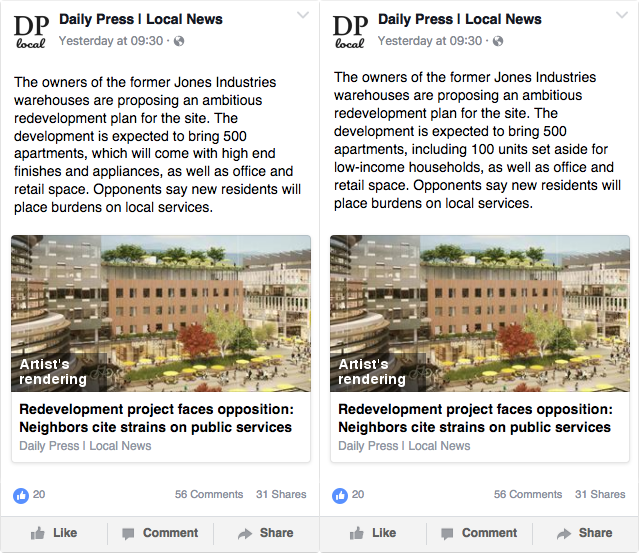
\includegraphics[width=.85\textwidth]{e_treatment}
  }
  \end{measuredfigure}
  \begin{tablenotes}[flushleft]
    \item \hspace{-.2em}\emph{Notes:} Respondents are shown a graphic for either the ``high-end'' project (left) or the mixed-income project (right). The graphic presents information about the project, as well as an artist's rendering of the proposed development.
  \end{tablenotes}
\end{figure}

Information about the project is presented as a Facebook post by a local news outlet.  This format allows for a short vignette to be presented together with a rendering of the proposed development in a realistic way; see Figure~\ref{fig:e_treatment}.\footnote{The artist's rendering is taken from documents filed by the developers of the pen factory project, described in Section~\ref{sec:introduction}.}  The text of the vignette reads:

\begin{quote}
The owners of the former Jones Industries warehouses are proposing an ambitious redevelopment plan for the site. The development is expected to bring 500 apartments, [which will come with high end finishes and appliances / including 100 units set aside for low-income households], as well as office and retail space. Opponents say new residents will place burdens on local services.
\end{quote}

The graphic primes respondents to consider the potential costs of the project by highlighting in the main text and in the rendering's caption that the new development may strain local public services. The vignette is identical for respondents in both treatment groups, except for the section enclosed within brackets.  Finally, respondents are reminded that

\begin{itemize}
  \item A Yes vote will allow developers to build 500 [luxury / mixed-income] apartments, as well as offices and shops.
  \item A No vote will allow developers to build office space and shops, but no new apartments.
\end{itemize}

The reminder emphasizes that the vote is not about whether there will be development -- in both cases, commercial development will proceed -- but whether the project will include residential uses.  Respondents are then asked to state if they will vote yes or no on the project on a four-point Likert scale, with a fifth ``Unsure'' option.  On the same page of the survey, they are asked to justify their decision ``in a few words.'' Although respondents are free to write as few or as many words as they like, the request for a justification encourages respondents to take an additional moment to consider their decision.\footnote{The median length of the open-ended response is 17 words.}

\subsubsection{Summary Statistics}

It is well known that the MTurk population differs from the general population on a number of dimensions \citep[see e.g.][]{huff_who_2015}.  Table~\ref{tab:e_summary_stats} reports demographic characteristics of the sample who completed the survey, and compares these summary statistics to the demographics of several major U.S. cities based on the 2012-2016 American Community Survey 5-year estimates.  The MTurk sample has more females and is younger than the populations of the selected cities, but is similar in some other respects. For example, 40 percent of respondents in the MTurk sample are homeowners, a number comparable to Los Angeles and San Francisco (37 percent of households), as well as Chicago (44 percent).  In terms of education attainment, 55 percent of the MTurk respondents have at least a 4-year college degree, a number higher than most cities, but comparable to San Francisco (53 percent).  Finally, 82 percent of respondents report household income of less than \$100,000, a figure comparable to Chicago (77 percent), Los Angeles (75 percent), and New York (73 percent).

\begin{table}
  \begin{threeparttable}
  \caption{Summary Statistics and Comparison to Major Cities}
  \label{tab:e_summary_stats}
  \footnotesize
  \begin{tabularx}{\textwidth}{lXXXXXX}
    \hline
     & Mturk & Boston & Chicago & LA & NYC & SF \\ \hline
  Female & 0.58 & 0.53 & 0.52 & 0.51 & 0.53 & 0.49 \\ 
    Age $<$ 35 & 0.53 & 0.47 & 0.38 & 0.36 & 0.35 & 0.35 \\ 
    Age $>$ 54 & 0.09 & 0.25 & 0.28 & 0.28 & 0.31 & 0.30 \\ 
    Homeowner & 0.40 & 0.35 & 0.44 & 0.37 & 0.32 & 0.37 \\ 
    No college education & 0.08 & 0.34 & 0.40 & 0.43 & 0.43 & 0.25 \\ 
    Some college education & 0.37 & 0.24 & 0.26 & 0.27 & 0.23 & 0.23 \\ 
    Has 4-year college degree & 0.41 & 0.24 & 0.21 & 0.20 & 0.21 & 0.33 \\ 
    Post-graduate degree & 0.14 & 0.17 & 0.13 & 0.10 & 0.13 & 0.20 \\ 
    Income $<$ \$60,000 & 0.55 & 0.51 & 0.57 & 0.56 & 0.53 & 0.37 \\ 
    Income between \$60-99,000 & 0.27 & 0.18 & 0.20 & 0.19 & 0.20 & 0.17 \\ 
    Income between \$100-\$149,000 & 0.11 & 0.15 & 0.12 & 0.12 & 0.13 & 0.17 \\ 
     \hline
  \end{tabularx}
  \begin{tablenotes}[flushleft]
    \item \hspace{-.2em}\emph{Notes:} Summary statistics for major cities are based on the American Community Survey 2012-2016 5-year estimates.
  \end{tablenotes}
  \end{threeparttable}
\end{table}

\subsection{Results}

\subsubsection{Measuring Liberalism and Localism} 

Responses to the twelve attitudinal statements were used to construct measures of liberalism and localism.  I convert the responses on the Likert agree-disagree scale to continuous variables ranging from 1 to 4, with ``No opinion'' given a value of 2.5.  Each variable is then scaled to have mean 0 and unit variance.  I then apply principal components analysis (PCA) on responses to the statements. PCA transforms a set of possibly correlated observed variables into a set of orthogonal latent variables, or principal components (PCs).  Each PC is a linear combination of responses to the attitudinal statements. The orthogonality of the PCs is a useful property of this method, given my conceptualization of liberalism and localism as political beliefs that are not systematically correlated with each other.

To give substantive meaning to the PCs, or latent variables, I inspect the factor loadings, or weights, for each of the statements.  I pay particular attention to the loadings for two families of statements.  The liberalism family includes the following statements:

\begin{itemize}
  \item The distribution of money and wealth in this country today is fair.
  \item The government should not concern itself with reducing the income difference between the rich and the poor.
  \item Our government should redistribute wealth through higher taxes on the rich.
  \item Everyone born in this country has an equal chance to succeed in life, whether their family is rich or poor.
\end{itemize}

The localism family includes the following statements:

\begin{itemize}
  \item Local government should focus on helping local businesses do well, rather than attracting new firms to the area.
  \item People who cannot afford their rent should move to somewhere cheaper, instead of asking the government for help.
  \item Every resident of a town or city should have an equal say on local issues, whether they just arrived or are long-time residents.
\end{itemize}

Liberalism and localism scores are the principal components that most heavily weigh responses in the respective families.  To understand what these scores mean substantively, I show how the scores correspond to raw responses to each attitudinal statement. For each attribute, liberalism and localism, I categorize respondents into  terciles based on their scores, and report the proportion of respondents in each tercile who agree or disagree with each statement.  The left column of Figure~\ref{fig:e_pc} reports the distributions conditional on liberalism scores.  Consider, for example, responses to the first statement, ``Our government should redistribute wealth through higher taxes on the rich.''  97 percent of respondents in the top liberalism tercile (those with the highest scores) agree with this statement, compared to 33 percent of respondents in the bottom tercile.  In contrast, 58 percent of respondents in the bottom liberalism tercile agree with the statement that ``The government should \emph{not} concern itself with reducing the income difference between the rich and the poor,'' compared to 1 percent of those in the top tercile. The conditional distributions of the responses demonstrate that liberalism scores differentiate respondents in favor of economic equity and redistributive economic and social policies from those opposed to such policies.

The right column of Figure~\ref{fig:e_pc} likewise reports the distributions conditional on the localism scores.  Respondents in the highest and lowest terciles for localism differ most significantly in their responses to statements in the localism family. For example, only 58 percent of respondents in the top tercile (highest localism score) agree that ``Every resident of a town or city should have an equal say on local issues, whether they just arrived or are long-time residents,'' compared to 94 percent of those in the lowest tercile.  Similarly, 91 percent of respondents in the top tercile agree that ``Local government should focus on helping local businesses do well, rather than attracting new firms to the area,'' compared to only 36 percent of those in the bottom tercile.  By contrast, the differences in the responses to statements in the liberalism family are relatively small.  69 percent of those in the top localism tercile agree that ``Our government should redistribute wealth through higher taxes on the rich,'' a proportion similar to the 71 percent of those in the bottom tercile who agree.

% Principal components

\begin{figure}[p]\centering
  \caption{Distribution of Attitudes across Liberalism and Localism Categories}
  \label{fig:e_pc}
  \begin{measuredfigure}
  \makebox[\linewidth]{%
  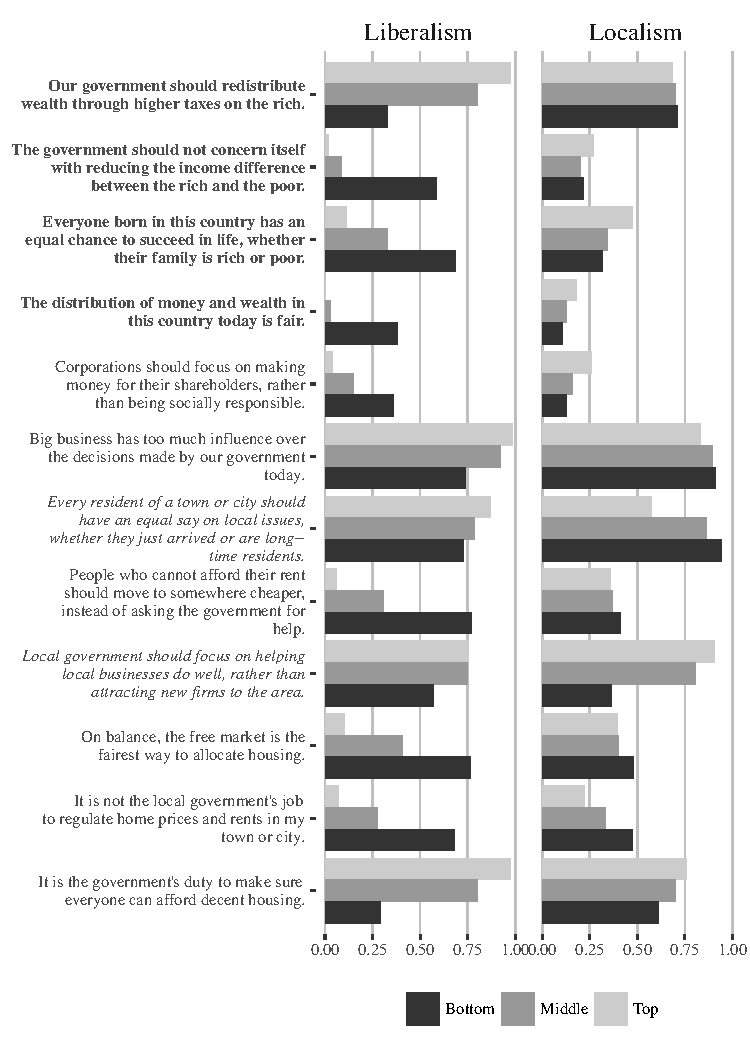
\includegraphics[width=.85\textwidth]{e_pc}
  }
  \end{measuredfigure}
  \begin{tablenotes}[flushleft]
    \item \hspace{-.2em}\emph{Notes:} The figure shows the proportion of respondents who agree with each statement, conditional on liberalism and localism score terciles.  Respondents at different ends of the liberalism scale are differentiated by responses to statements about economic equality and redistribution (in bold). Respondents at different ends of the localism scale are differentiated by responses to statements about local community (in italics). 
  \end{tablenotes}
\end{figure}

Note that the type of localism captured by this principal component does not necessarily incorporate a heightened concern for exclusion.  36 percent of respondents in the top localism tercile agree that ``People who cannot afford their rent should move to somewhere cheaper, instead of asking the government for help,'' only marginally lower than the 41 percent in the bottom tercile who agree.\footnote{The statement about whether ``people who cannot afford their rent should move to somewhere cheaper, instead of asking the government for help'' was grouped in the localism family, to tap respondents' support for public policies to reduce gentrification-driven displacement.  However, responses turned out to be more correlated with statements in the liberalism family, suggesting respondents interpreted the statement as being related to a more general question about state intervention to solve a social problem.  Indeed, aside from the two questions about ``equal say'' and ``local businesses'', most statements load on the liberalism PC.}  Because principal components are orthogonal to each other by construction, those who score high (or low) on localism are neither more nor less economically liberal than others. Rather, localism appears to reflect the belief that locals -- long-time residents and legacy businesses -- should be given priority over newcomers and outsiders, whether in terms of political voice or economic development initiatives.  

Table~\ref{tab:e_lib_loc_regression} presents estimates for linear regressions of liberalism and localism on gender, race, age, education, income, and housing status. I note in particular that not having a college degree is positively associated with localism.  On its face, this finding could be explained by geographical mobility.  That is, respondents with higher education attainment may be less likely to express localist attitudes because they are more geographically mobile.  However, other indicators of geographical mobility, such as income, homeownership, or whether the respondent is a long-time resident in her current town or city, are not associated with localism. Taken together, these results suggest that localism may be driven by cultural or ideational mechanisms in a manner analogous to the formation of attitudes toward immigration \citep[see e.g. the discussion in][]{hainmueller_public_2014}. To be clear, I do not claim that localism is like holding anti-immigration attitudes. Rather, I conjecture that localism is a type of ideational or cultural belief, not an expression of economic self-interest.

% Predictors

\begin{table}
  \caption{Predictors of Liberalism and Localism}
  \label{tab:e_lib_loc_regression}
  \begin{threeparttable}
  \footnotesize
  \begin{tabularx}{\linewidth}{X}
  \centering

  \begin{tabular}{@{\extracolsep{5pt}}lcc} 
  \\[-1.8ex]\hline 
  \hline \\[-1.8ex] 
   & \multicolumn{2}{c}{\textit{Dependent variable:}} \\ 
  \cline{2-3} 
  \\[-1.8ex] & Liberalism & Localism \\ 
  \\[-1.8ex] & (1) & (2)\\ 
  \hline \\[-1.8ex] 
   Female & 0.454$^{}$ & 0.088$^{}$ \\ 
    & (0.095) & (0.044) \\ 
    & & \\ 
   White & $-$0.186$^{}$ & $-$0.300$^{}$ \\ 
    & (0.111) & (0.052) \\ 
    & & \\ 
   Age < 35 & 0.197$^{}$ & 0.242$^{}$ \\ 
    & (0.101) & (0.047) \\ 
    & & \\ 
   No 4-year college degree & $-$0.266$^{}$ & 0.173$^{}$ \\ 
    & (0.103) & (0.048) \\ 
    & & \\ 
   Post-graduate degree & 0.053 & $-$0.089 \\ 
    & (0.146) & (0.068) \\ 
    & & \\ 
   Income < \$60,000 & 0.306$^{}$ & 0.077 \\ 
    & (0.115) & (0.053) \\ 
    & & \\ 
   Income \$100-150,000 & $-$0.280$^{}$ & $-$0.025 \\ 
    & (0.163) & (0.076) \\ 
    & & \\ 
   Income > \$150,000 & $-$0.434$^{}$ & $-$0.167 \\ 
    & (0.251) & (0.117) \\ 
    & & \\ 
   Homeowner & $-$0.616$^{}$ & $-$0.074 \\ 
    & (0.107) & (0.050) \\ 
    & & \\ 
   Resident > 4 years & 0.165 & 0.062 \\ 
    & (0.103) & (0.048) \\ 
    & & \\ 
   5-year HPA > median & 0.163$^{}$ & 0.021 \\ 
    & (0.096) & (0.045) \\ 
    & & \\ 
   Constant & $-$0.151 & $-$0.071 \\ 
    & (0.193) & (0.090) \\ 
    & & \\ 
  \hline \\[-1.8ex] 
  Observations & 1,941 & 1,941 \\ 
  R$^{2}$ & 0.062 & 0.064 \\ 
  Adjusted R$^{2}$ & 0.056 & 0.059 \\ 
  \hline 
  \hline \\[-1.8ex] 
  \end{tabular} 

  \end{tabularx}
  \begin{tablenotes}[flushleft]
    \item \hspace{-.2em}\emph{Notes:} OLS estimates of linear models for liberalism and localism.  Base category for education is 4-year college degree; base category for income is \$60-100,000; median 5-year home price appreciation (HPA) is based on Zillow data, median of 100 largest cities. ``Resident > 4 years'' means respondent has lived in the current town or city for 5 or more years.
  \end{tablenotes}
  \end{threeparttable}
\end{table}

\subsubsection{Support for Redevelopment Projects}

Before turning to the relationship between support for redevelopment projects and political beliefs, I discuss a simple model of support in which voters prefer the type of project (high-end or mixed-income apartments) that maximizes narrow economic benefits for themselves.  In this model, renters at each income level prefer the project type that produces more housing units at their income level.  The reason is that an increase in the supply of housing units in a given market segment decreases rents for that type of housing.  This model would hence predict that lower-income renters prefer the mixed-income project over the high-end apartments, whereas high-income renters would prefer the converse.  Homeowners prefer the project type that leads to a greater increase in home prices.  All else equal, homeowners across income groups should not differentially prefer one project type over another.  Suppose, however, that lower-income homeowners live in neighborhoods with lower home prices, compared to the neighborhoods in which high-income homeowners live. Then, lower-income homeowners should prefer the project with 100 percent high-end apartments over the mixed-income project, to the extent that the high-end project has a greater positive impact on local property prices, compared to the mixed-income project.  Another reason lower-income homeowners might prefer the high-end project is that the mixed-income project would introduce new low-income housing units into the neighborhood and depress home prices in the lower-income market segment.

Figure~\ref{fig:e_income_tenure} reports support for each project type among non-owners (renters) and owners across three income groups.  Support is defined as choosing ``Definitely yes'' or ``Probably yes'' for the vote choice question.  High-income renters are more likely to support the high-end project, compared to lower-income renters.  However, contrary to the predictions of the model sketched out above, renters at every income level prefer the mixed-income project to the high-end project.  Lower-income homeowners are also more likely to support the mixed-income project.  Among homeowners, the relative preference for the mixed-income project decreases with income.  The difference in support for the two projects among high-income homeowners is statistically indistinguishable from zero.  Of course, more elaborate theories based on narrow economic self-interest could explain the heterogeneous treatment effects observed. My argument is that a parsimonious model based on political beliefs can capture meaningful variation in support for redevelopment projects in a way that a parsimonious model based on narrow economic self-interest cannot.

% Figure: Income and tenure. Inconsistent with narrow self-interest.

\begin{figure}[tb]\centering
  \caption{Support for Project by Household Income and Tenure}
  \label{fig:e_income_tenure}
  \begin{measuredfigure}
  \makebox[\linewidth]{%
  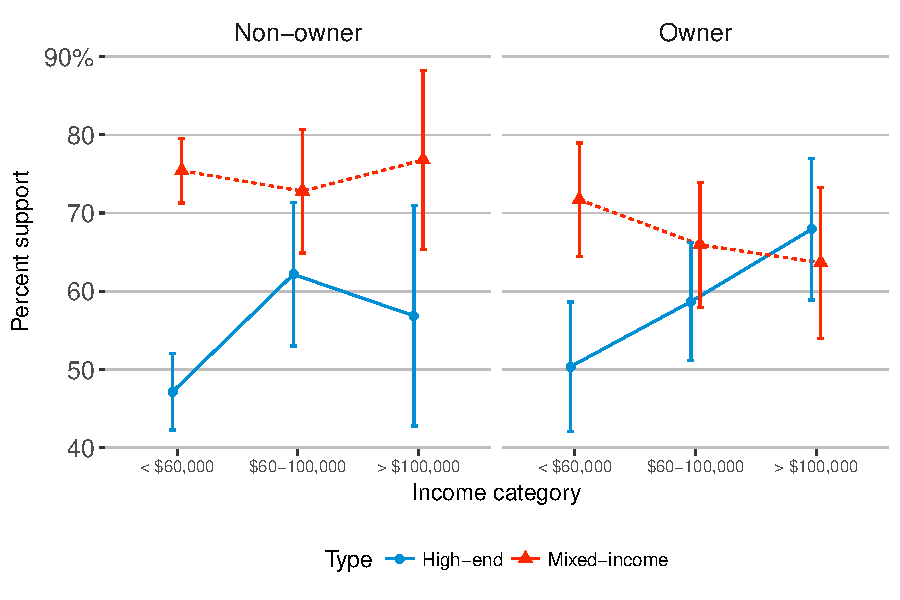
\includegraphics[width=.85\textwidth]{e_income_tenure}
  }
  \end{measuredfigure}
  \begin{tablenotes}[flushleft]
    \item \hspace{-.2em}\emph{Notes:} The figure shows the proportion of respondents that support each project type, for each income category within each housing tenure type (non-owners and homeowners). Error bars indicate 95\% confidence intervals.
  \end{tablenotes}
\end{figure}


Data from the survey experiment exhibit patterns consistent with the theory discussed in Section~\ref{sec:theory}.  As Figure~\ref{fig:e_lib_loc} shows, support for the mixed-income project increases with liberalism (left panel). The predicted probability of supporting the mixed-income project increases from 60 percent for a voter with a liberalism score at the 20th percentile, to 82 percent for a voter with a liberalism score at the 80th percentile, an increase of 22 percentage points.\footnote{Predicted probabilities are computed based on a loess fit.}  The positive association between liberalism and support for the  project is reversed when the apartments are all high-end.  As a result, the treatment effect (i.e. the relative preference for the mixed-income over the high-end project) increases from -1 percentage point (statistically insignificant) to 39 percentage points over the same range of liberalism. Among liberal voters, lower-income set-asides have a substantively and statistically significant effect on support for redevelopment with a residential component. Where only a minority of liberal voters support the mixed-use over the commercial-only project when all apartments are marketed as high-end, an overwhelming majority of such voters support the project when units are set aside for lower-income households.

% Figure: Bivariate loess, liberalism and localism (hetero. treatment efx for lib, decr. support for loc.)

\begin{figure}[tb]\centering
  \caption{Support for Project by Liberalism and Localism Scores}
  \label{fig:e_lib_loc}
  \begin{measuredfigure}
  \makebox[\linewidth]{%
  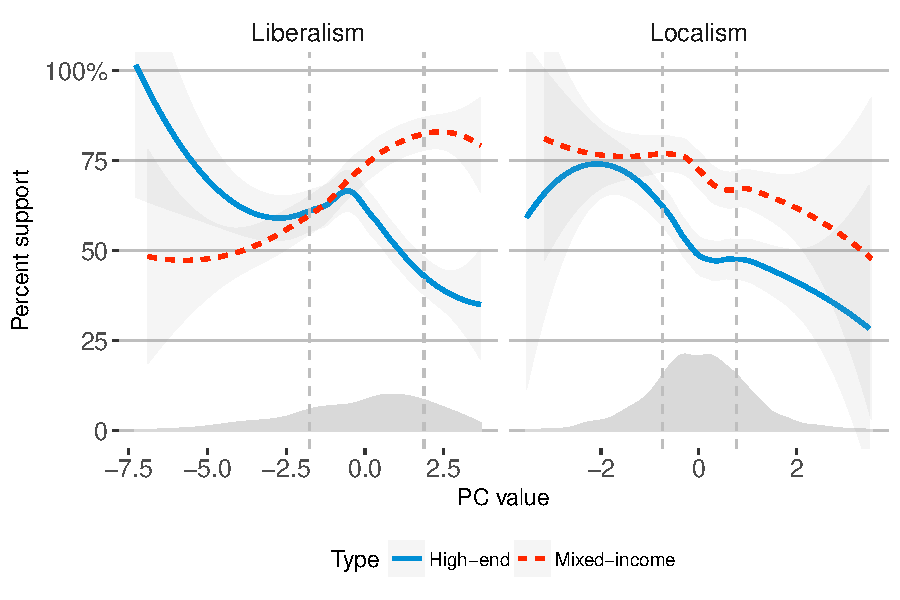
\includegraphics[width=.85\textwidth]{e_lib_loc}
  }  
  \end{measuredfigure}
  \begin{tablenotes}[flushleft]
    \item \hspace{-.2em}\emph{Notes:} The figure shows the bivariate relationship between respondents' support for each project type, and liberalism and localism scores. Lines are loess curves.  Density curves at the bottom of the plots show the distribution of the scores; note that the probability densities are scaled for aesthetic reasons and do not correspond to the tick marks on the y-axis. Shaded areas indicate 95\% confidence intervals. The vertical dashed lines represent the 20th and 80th percentiles for the respective scores.
  \end{tablenotes}
\end{figure}

In contrast to liberalism, localism is negatively associated with support for both mixed-income and high-end projects.  The predicted probability of supporting the mixed-income project decreases from 77 percent for a voter with a localism score at the 20th percentile, to 67 percent for a voter with a liberalism score at the 80th percentile, a decline of 10 percentage points.   Likewise, the probability of supporting the high-end project decreases from 62 percent to 48 percent over the same range, or a decline of 14 percentage points.  While it is not a prediction made by the model, it is intriguing that voters at the extreme low end of the localism scale do not appear to discriminate between the types of project.  For example, at the 1st percentile of localism, the predicted probability of supporting the mixed-income project is 77 percent, compared to 74 percent for the high-end project, a difference of 3 percentage points not statistically distinguishable from zero at the 95\% confidence level; see Figure~\ref{fig:e_ate}.  Non-localists -- respondents who tend to be open to both newcomers and new businesses -- are equally happy to support both high-end and mixed-income developments. The finding is consistent with the expansive view of ``community'' espoused by proponents of residential development at all income levels.

% Liberalism and localism indexes

The estimated relationships between support for the projects and liberalism and localism may be confounded by unobserved variables. For example, the positive association between support for a mixed-income project and liberalism may simply reflect the effect of income, if lower-income individuals tend to be more liberal.  I estimate linear models of support for each type of project, controlling for gender, race, age, education, income, housing tenure, and local home price appreication.  Figure~\ref{fig:e_lib_loc} suggests that the relationships between support and liberalism and localism can be approximated with a quadratic function, so I include squared terms for liberalism and localism in the models.  Table~\ref{tab:e_support_regression} shows that the associations between political beliefs and support for each project type are robust to the inclusion of covariates.

% Figure: Contour, H and M

\begin{figure}[t]
  \caption{Contour Plots of Support for Project by Project Type}
  \label{fig:e_contour}
  \begin{measuredfigure}
  \makebox[\linewidth]{%
  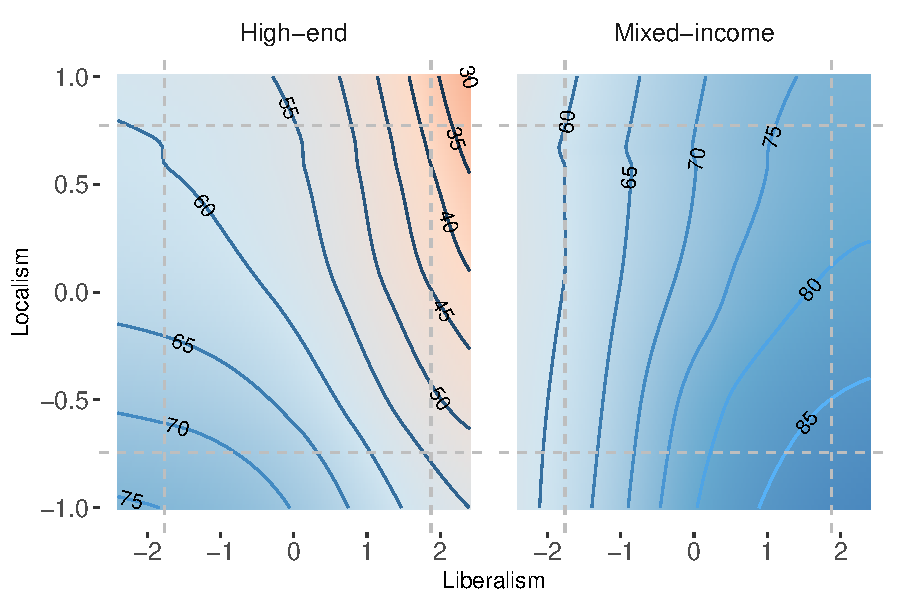
\includegraphics[width=.85\textwidth]{e_contour}
  } 
  \end{measuredfigure}
  \begin{tablenotes}[flushleft]
    \item \hspace{-.2em}\emph{Notes:} The figure shows predicted support for each type of project (high-end or mixed-income housing) as a function of a respondent's liberalism and localism scores, based on loess fits with the two predictors.  The vertical and horizontal dashed lines represent the 20th and 80th percentiles for liberalism and localism scores, respectively.
  \end{tablenotes}
\end{figure}

Figure~\ref{fig:e_contour} reports the combined effect of liberalism and localism on support for each type of project.  Like Figure~\ref{fig:e_lib_loc}, the plots report the predicted probabilities of support for a project based on loess fits; the difference is that in these plots, support is modelled as a function of both liberalism and localism.  The figure shows that liberal localists are least supportive of the high-end project (top right corner of the left panel), whereas liberal non-localists are most supportive of the mixed-income project (bottom right corner of the right panel). 

More interestingly, the plots show how localism is differentially associated with support for the projects conditional on liberalism. Consider the predicted probabilities of support for the high-end project.  Among respondents at the 20th percentile of liberalism (left vertical line), moving from the 20th to 80th percentile of localism (from the bottom to the top horizontal line) decreases support for the project from 72 to 60 percent, a decline of 12 percentage points. Among respondents at the 80th percentile of liberalism (right vertical line), support decreases from 54 to 38 percent, a decline of 16 percentage points. The localism gradient of support for the high-end project is steeper among liberals than conservatives (the same is true for the mixed-income project).  Localism is an especially potent force in shaping attitudes toward development in liberal cities, because high land and construction costs orient private development toward high-end (or market-rate) development, and localism can tip the scale away from support for development.

\subsection{Discussion}

Political economy models of housing growth preferences derive individuals' preference for growth from their interests with respect to home prices.  In this section, I show how preferences can also be shaped by individuals' political beliefs.  I focus on two types of beliefs that I call liberalism and localism.  I show that the treatment effect of a mixed-income project -- that is, the relative preference for a mixed-income project over a high-end project -- is positive and substantively large among liberals, but small and statistically insignificant among conservatives (and negative among very conservative individuals).  Support for both types of projects decreases with localism. The treatment effect of the mixed-income project is positive across most values of localism, but respondents with low localism scores tend to be supportive of both projects.

A concern about the survey experiment is that it does not use actual behavior as its outcome variable.  Survey respondents may support or oppose a project simply as a way to express underlying attitudes, given that there are no real-life costs or benefits at stake.  The next section attempts to bridge the gap between reported preferences and actual behavior by studying voting outcomes in a city  where liberalism and localism are shaping responses to a housing affordability crisis.

\section{San Francisco's Land Use Ballot Measures, 2000-2016}\label{sec:sf}

A report published by California's Legislative Analyst's Office in 2015 enumerated the causes of housing supply shortfalls in the state's coastal areas, beginning with ``Community Resistance to New Housing'' \citep{alamo_californias_2015}.  The report highlighted the effect of local ballot measures on limiting development, noting that ``California's high degree of voter involvement in land use decisions appears to be unique'' (p. 17).  In this section I exploit rich elections data on housing and land use ballot measures in California.  I focus on one city, San Francisco, where voters have repeatedly gone to the polls to make decisions on land use.  The goals of this study are to discover the latent structure of political preferences that undergirds observed vote outcomes, ascertain if any dimensions of this structure can be plausibly described as liberalism and localism, and finally estimate the association between these latent factors and support for redevelopment projects.

\subsection{Setting}

\subsubsection{Housing and Land Use Ballot Measures}

California's state constitution empowers its cities to pass ordinances on traditional municipal matters without prior authorization from the state legislature, to the extent that such ordinances do not conflict with a general state law (Article XI, section 7).  The empowerment of localities by the state to pass laws and ordinances without a prior delegation of authority from the state is known as home rule, and the basis for such laws and ordinances is founded in local police power, which gives local governments the right to act in a way that promotes the health, safety, and general welfare of the community.\footnote{See for example the discussions in \citet[pp.19ff]{fischel_homevoter_2001} and \citet[pp.70ff]{berman_local_2015}.}  Land use regulation, in particular, has its basis in police power.  

Citizens can influence local public policies in several ways.  They can elect or lobby public officials.  In some states, including California, they can also petition to place legislation on the ballot to be voted on directly by the electorate.  The same process also allows citizens to repeal legislation passed by elected officials.  In California, the use of such initiatives and referenda to shape local land use planning, a phenomenon known colloquially as ``ballot box zoning,'' began in the 1970s \cite[p.244]{fulton_guide_2012}.  Initiatives restricting growth first appeared on local ballots in the San Francisco area, but gradually spread to localities in Southern California over the course of the 1970s and 1980s.

The most common type of land use measures restrict or ease restrictions on development.  For example, Proposition M in San Francisco's 1986 November elections placed an annual cap on the square footage of office space in high-rise buildings; subsequent measures have sought to amend this cap.  Measures could also seek to impose development moratoriums in certain neighborhoods.  Other measures have more subtle effects on growth. For example, parking requirements stipulate the minimum number of parking spaces developers would need to include in new projects. Reduced minimum parking requirements, especially in neighborhoods well served by public transit, can reduce per-unit costs for developers, increase housing density, and help improve housing affordability. Measures that seek to amend parking requirements thus have a subtle but direct effect on housing growth.

A second type of measures introduces or amends procedural barriers to development. Such measures might mandate voter approval for zoning changes or increases to height limits.  Conversely, a measure might require the city to let a project proceed so long as it meets certain criteria, allowing the project to circumvent hearings, appeals, and petitions.  Another example would be a measure that mandates publicly-funded projects, such as affordable housing developments, to receive a minimum number of bids or proposals. To the extent that such projects are complex and require specialized expertise, such a mandate may limit the number of types of projects that can be built.

A third type of ballot propositions are fiscal measures. Such measures could require that a proportion of tax revenues be set aside for specific uses, such as acquiring or preserving open space, affordable housing, and so on.  These measures do not raise new revenue, but provide dedicated funding sources for certain public projects. Voter approval is also needed for bond issues. Over the last two decades, San Francisco voters have gone to the polls thrice -- in 2002, 2004, and 2015 -- to approve new bond issuance to fund affordable housing programs.

A fourth type of propositions relate to voter approvals for specific projects. These projects are described in more detail in the following section.  The specifics of each project require additional exposition because of our theorizing that citizens' political beliefs are differentially associated with support for redevelopment, depending on the characteristics of each redevelopment project.

\subsubsection{Redevelopment Projects}\label{sec:g_redev}

Since 2008, San Francisco's voters have voted on six measures related to approvals for four redevelopment projects. Figure~\ref{fig:g_devs} indicates the locations of these projects. The projects were the subjects of ballot measures either because local legislation require voters to approve zoning or height limit changes in specific situations (as with the Hunters Point Shipyard, Pier 70, and Mission Rock), or because proponents or opponents -- or both -- collected sufficient signatures for a petition to put a measure on the ballot (as with the 8 Washington project).  I describe the projects in more detail below, noting in particular whether each project was perceived as being sufficiently attentive to housing affordability or not.

\begin{figure}[tb]\centering
  \caption{Project-specific Ballot Measures}
  \label{fig:g_devs}
  \begin{measuredfigure}
  \makebox[\linewidth]{%
  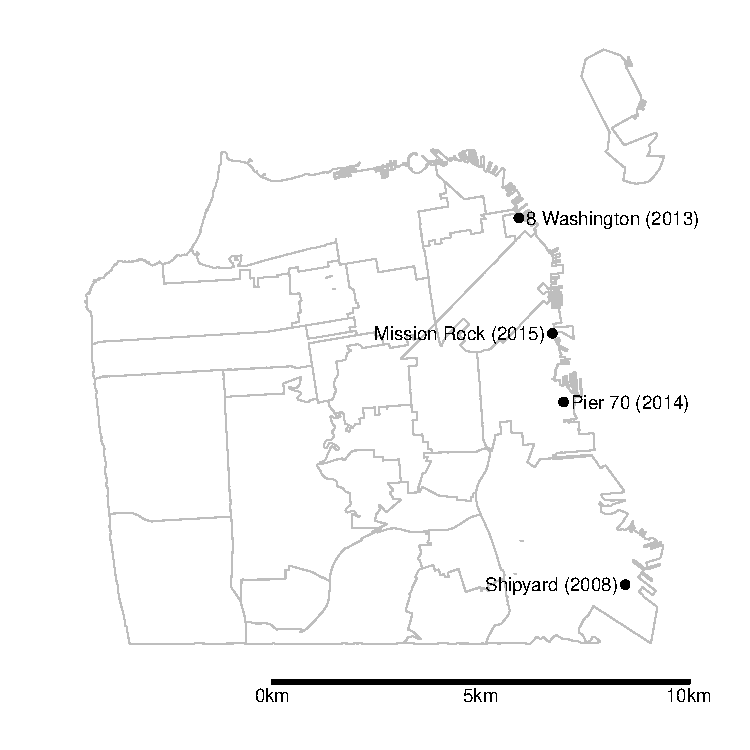
\includegraphics[width=.9\textwidth]{g_devs}
  }
  \end{measuredfigure}
  \begin{tablenotes}[flushleft]
    \item \hspace{-.2em}\emph{Notes:} The figure shows the locations of four projects that sought voter approval between 2008 and 2015.
  \end{tablenotes}
\end{figure}

\paragraph{Hunters Point Shipyard.} In June 2008, San Francisco voters voted on a proposed framework for the redevelopment of the Hunters Point Naval Shipyard and Candlestick Point (Measure G). The proposition was placed on the ballot because the site included an existing stadium, which together with its surrounding parking lots were classified as open space; city laws require voter approval to change the zoning of open space for other uses. The mayor further decided to expand the scope of the ballot measure to seek a broad mandate for the redevelopment of the site. The proposal envisioned the production of 8,500 to 10,000 new housing units. The proposition text did not, however, specify the affordability levels of these units.\footnote{A Community Benefits Agreement signed by the developer and community organizations in May 2008 committed the developer to pricing at least 32 percent of units at affordable levels. See \url{https://d10benefits.org/wp-content/uploads/2013/01/lennar_ad10_ccba_executed-1.pdf}.} The language of Measure G was perceived by some as being relatively favorable to developers.\footnote{San Francisco distributes voter pamphlets to voters that contain arguments and endorsements contributed by each proposition's proponents and opponents. In their official argument against Measure G, opponents begin with the claim that ``Proposition G makes big promises but doesn't guarantee affordable housing, jobs for local residents, or any more parkland than already exists. Proposition G is a sweetheart deal for Lennar, an out-of-state developer that has already spent over \$1,000,000.00 on its political campaign. \ldots{}. Transit `improvements' promised by Lennar will primarily benefit new luxury condo owners, not the rest of Bayview.''}  Partly in response to perceived slipperiness in Measure G as regards the project's commitment to housing affordability, opponents to the project gathered sufficient signatures to place a competing measure on the ballot (Measure F). The competing measure required the project to set aside at least 50 percent of new housing units as affordable housing, with varying levels of affordability benchmarked to median household income in the city. Measure G passed with 63 percent of the vote; Measure F failed with 37 percent. About 160,000 votes were cast.

\paragraph{8 Washington.} In 2012, the San Francisco Board of Supervisors passed an ordinance that increased height limits for a triangular site on the city's eastern waterfront, as part of the approvals for a recreational, retail, and residential development known as 8 Washington Street. A private recreation club and a parking lot owned by the Port of San Francisco were (and continue to be) located at the site. Local law provides for citizens to reaffirm or overturn the Board's decision in a referendum, and opponents of the height limit increases gathered sufficient signatures to put the question to voters in the November 2013 local elections (Measure C). Although Measure C was narrowly focused on the question of height limits, overturning the height limit increases would effectively prevent the project from proceeding. In response, proponents of the project put a competing measure on the ballot (Measure B) for voters to approve the project.  The project as proposed would have added 134 market-rate units to the housing stock. In addition, the developer pledged a \$11 million contribution to the city's affordable housing fund. Although opponents' main complaint addressed the height limit increase, they also noted the absence of on-site affordable housing, and claimed that the new ``luxury condos'' would cost \$5 million on average.  About 125,000 votes were cast, and the project was rejected by about 65 percent of voters. The developer abandoned the project in 2016.

\paragraph{Pier 70 and Mission Rock.} In June 2014, voters passed a ballot measure mandating voter approval for height limit increases on certain sites along the eastern waterfront. The measure directly affected two developments, Pier 70 and Mission Rock.  The developer for the Pier 70 project, which had been engaging interest groups and community members on its plans for the site since 2011, felt sufficiently confident in its level of community support to put the project on the November 2014 ballot \citep{kuwada_shaping_2015}.\footnote{Incidentally, Forest City is the developer for Pier 70 -- the same firm that developed University Park, described at the beginning of Section~\ref{sec:exp}.} The project would add between 1,000 and 2,000 housing units to the city, with the developer committing to price 30 percent of the units at levels affordable to low- and middle-income households. The proportion of affordable housing units exceeded the 12 percent affordable requirement that was city law at the time. The Mission Rock project, which was on the November 2015 ballot, committed to an even higher proportion of affordable housing. The project envisioned 1,000 to 1,950 new housing units, of which at least 40 percent would be affordable to low- and middle-income households. Endorsements of the two measures published in official voter pamphlets underline the high proportion of affordable housing units proposed for these two projects.  Both measures won at the ballot box with similar margins -- 73 to 74 percent `Yes' votes -- and over 200,000 votes cast.

\subsection{Data and Measurement}

\subsubsection{Dataset}

I construct a novel panel dataset of voting outcomes for about 600 precincts in San Francisco, California, on 38 city-level housing and land use related ballot measures presented to voters between 2000 and 2016. The set of measures used in the analysis was defined by including all measures belonging to the ``land use'' category as coded by researchers for the California Elections Data Archive, a project co-sponsored by the Office of the California Secretary of State.\footnote{The project's website is at \url{http://www.csus.edu/isr/projects/ceda.html}.} The initial list of measures was then supplemented by measures that included the words ``land'' or ``development'' and are clearly related to land use. The latter set of measures mostly relate to affordable housing issues and approvals for specific projects.

The San Francisco Department of Elections publishes vote counts for each ballot proposition at the precinct level. In 2016, about 850 voters were registered in each precinct on average. Because precinct boundaries change from election to election, I create a panel by matching precincts from a reference election (specifically the 2012 general election) to precincts from other elections based on the proportion of spatial overlap between precincts. In other words, each precinct from the 2012 general elections is matched to a precinct in every other elections to create the panel.

\subsubsection{Measures of liberalism and localism}

Similar to the study in Section~\ref{sec:exp}, I apply principal components analysis to the observed precinct-level vote outcomes to generate uncorrelated latent dimensions. I included 32 ballot measures in the PCA, leaving out the 6 redevelopment project measures discussed above.  I then inspect the loadings for each PC to determine if any of the PCs can be plausibly interpreted as measuring liberalism or localism.  Consistent with prior research in American political behavior, the first PC has a clear interpretation as a measure of liberalism \citep[e.g.][]{ansolabehere_candidate_2001-1,tausanovitch_measuring_2013}.  

To illustrate the substantive interpretation of this latent dimension, I categorize precincts into terciles according to their liberalism scores, and report the average vote share by terciles for a selected set of ballot measures.  High liberalism precincts are differentiated from low liberalism precincts by mean vote shares for ballot measures that are redistributive in nature.  Consider the ``Housing Trust Fund'' proposition (2012 November Proposition C), which sets aside a portion of the city's discretionary budget for affordable housing programs (Figure~\ref{fig:g_pc}, sixth row).  The average vote share in support for the measure was 75 percent among precincts in the top liberalism tercile, compared to 55 percent among those in the bottom tercile.  Support for ``Affordable Housing Bonds'' (2002 November Proposition B) was 71 percent among precincts in the top liberalism tercile, and 42 percent among those in the bottom tercile, a gap of nearly 30 percent.  The difference in vote shares between high and low liberalism precincts can also be observed in non-fiscal measures.  For example, Proposition R in the 2002 November elections proposed an easing of restrictions on converting rental apartments to condominiums, a policy that was perceived to disadvantage lower-income households by moving apartments out of the rent-controlled housing stock.  The average `Yes' vote share was 29 percent among precincts in the top liberalism tercile, substantially lower than the 49 percent among those in the bottom tercile (Figure~\ref{fig:g_pc}, third row from bottom).

\begin{figure}[p]\centering
  \caption{Support for Ballot Propositions across Liberalism and Localism Categories}
  \label{fig:g_pc}
  \begin{measuredfigure}
  \makebox[\linewidth]{%
  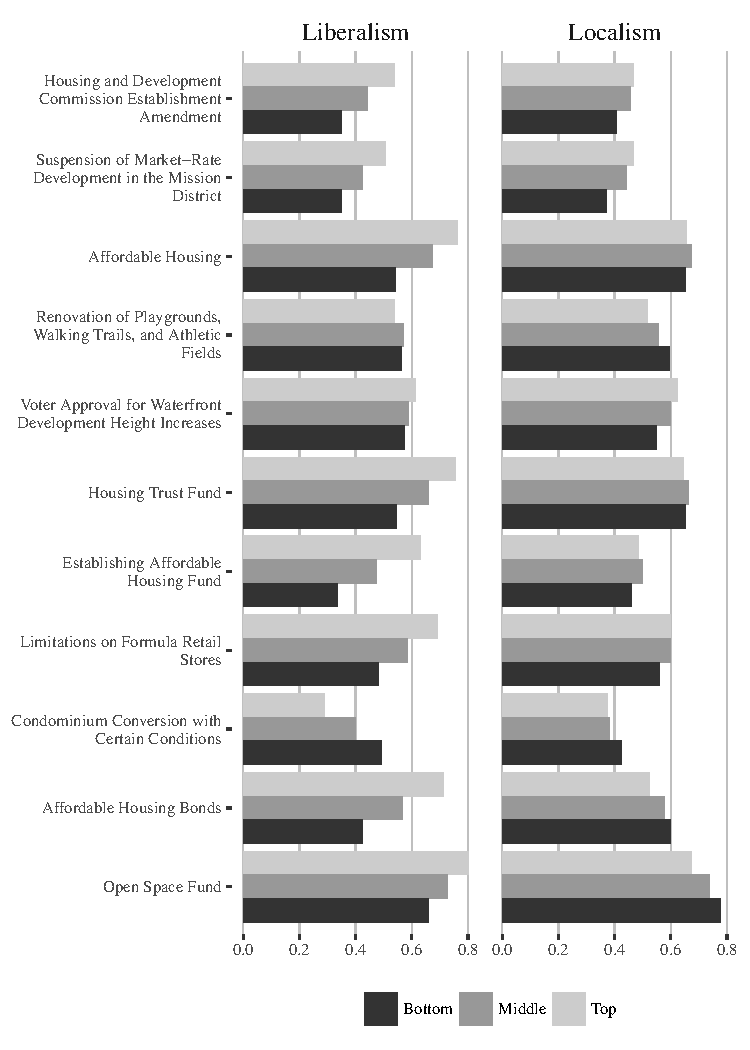
\includegraphics[width=.85\textwidth]{g_pc}
  }
  \end{measuredfigure}
  \begin{tablenotes}[flushleft]
    \item \hspace{-.2em}\emph{Notes:} The figure shows the mean precinct-level vote in favor of each ballot proposition, conditional on liberalism and localism score terciles.
  \end{tablenotes}
\end{figure}

To identify a latent dimension associated with localism, I inspect the loadings to find the PC that best differentiated precincts on ballot measures that limit or enhance voter control over development.  These measures include November 2014 Measure I, which limits local residents' ability to block improvements to recreational facilities that would at least double the usage of a facility, as well as the aforementioned June 2014 Measure F, which mandates voter approval for height limit increases on certain sites along the eastern waterfront.  Based on this criterion, I select the third PC as a measure of localism. Although this PC explains significantly less variance in the observed vote outcomes compared to the liberalism dimension, it can still be differentiated from subsequent PCs in terms of the proportion of variance explained (see Figure~\ref{fig:g_scree}).  Among precincts in the top localism tercile, the average vote share in support of the ``Renovation of Playgrounds'' measure was 52 percent, compared to 60 percent in the bottom tercile (recall that this measure would \emph{limit} the ability of local communities to challenge certain public works improvements).  Localism also differentiates precincts on the ``Voter Approval for Waterfront Development Height Increases'' measure, for which mean vote shares were 62 and 55 percent for the top and bottom localism terciles respectively.  Conversely, the localism dimension does not differentiate precincts for redistributive ballot propositions.  Among precincts in the top localism tercile, the average vote share in support of the ``Housing Trust Fund'' measure was 64 percent, compared to 65 percent in the bottom localism tercile.  In short, precincts with high localism scores are more supportive of measures that enhance local community influence over development, and more opposed to measures that would limit such control.

The plots in Figure~\ref{fig:g_pc_map} report the values of the liberalism and localism scores for each precinct on a map of San Francisco. The geographic distribution of liberalism (top panel of figure) is consistent with qualitative descriptions of San Francisco's political geography. Observers of the city's politics refer to a ``Conservative C'' that stretches along the wealthy northern edge of the city, bordering the Presidio, down the middle- and upper-class west-side, and along the southern border.\footnote{See for example \url{http://www.dailykos.com/story/2012/11/19/1160963/-A-crash-course-in-San-Francisco-politics}.} Neighborhoods in the center of the city and toward the southeastern edge -- the ``Progressive Core'' -- are on the other ideological pole. Even in a city known for its liberal politics, substantive geographical variation exists with respect to preferences over redistributive public policy.

\begin{figure}\centering
  \caption{Geographical Distribution of Liberalism and Localism}
  \label{fig:g_pc_map}
  \begin{measuredfigure}
  \makebox[\linewidth]{%
  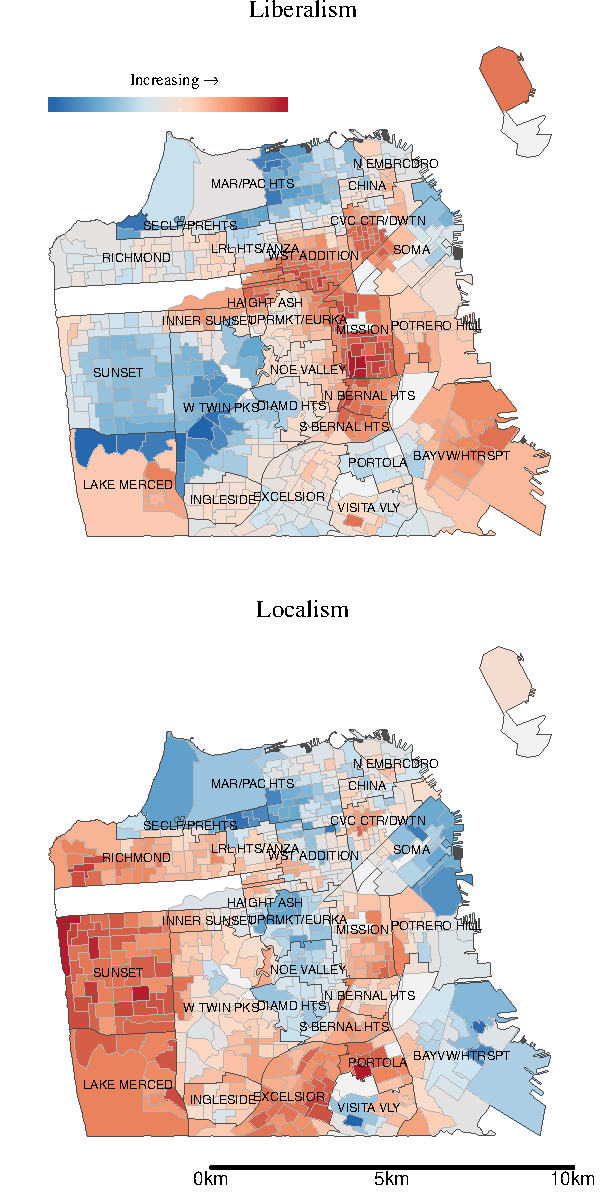
\includegraphics[width=.7\textwidth]{g_pc_map}
  }
  \end{measuredfigure}
  \begin{tablenotes}[flushleft]
    \item \hspace{-.2em}\emph{Notes:} The maps show the liberalism and localism scores for each precinct in San Francisco.
  \end{tablenotes}
\end{figure}

The geographical configuration of political preferences changes when we turn to localism (bottom panel of figure).  Neighborhoods on different ends of the liberalism spectrum can become proximate in terms of localism.  The Mission district, one of the most liberal neighborhoods, looks more similar to the conservative Sunset district on the localism dimension than its liberal neighbors in Noe Valley and the Castro (labelled as \texttt{EURKA} on the map, for Eureka Valley).  Categorizing San Francisco's neighborhoods along two dimensions -- liberalism and localism -- facilitates a richer understanding of the city's political geography.  Figure~\ref{fig:g_map_types} shows the clustering of neighborhoods based on the interaction of whether they score above or below the median on liberalism (liberal or conservative) and whether they score above or below the median on localism (localist or non-localist).  The theory described in Section~\ref{sec:theory} implies that support for redevelopment projects should vary systematically across the four different categories of neighborhoods.

\begin{figure}[tb]\centering
  \caption{Geographical Distribution of Political Preferences}
  \label{fig:g_map_types}
  \begin{measuredfigure}
  \makebox[\linewidth]{%
  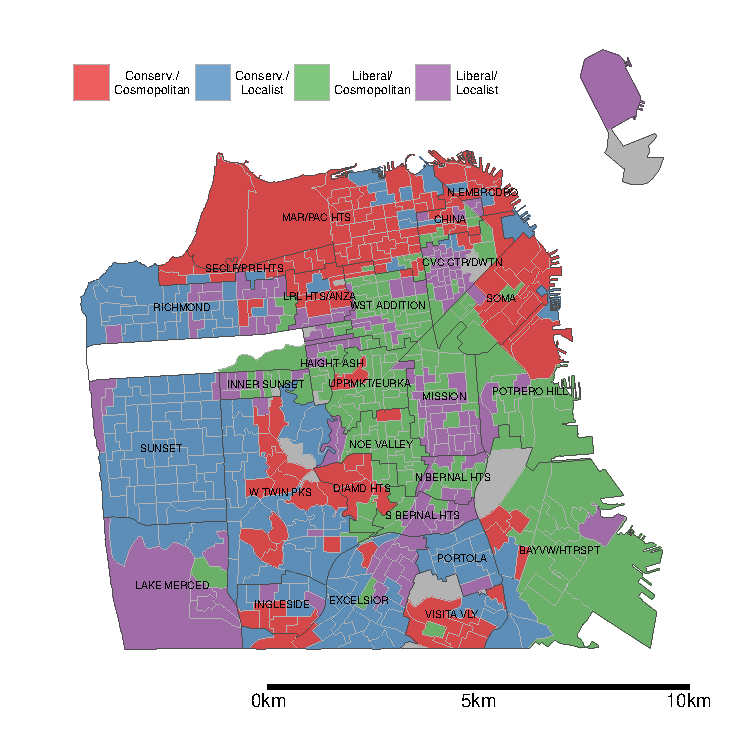
\includegraphics[width=.7\textwidth]{g_map_types}
  }
  \end{measuredfigure}
  \begin{tablenotes}[flushleft]
    \item \hspace{-.2em}\emph{Notes:} The map show the geographical distribution of four categories of political preferences. Precincts are categorized by the interaction of whether they score above or below the median on liberalism (liberal or conservative) and whether they score above or below the median on localism (localist or non-localist).
  \end{tablenotes}
\end{figure}

\subsection{Support for Redevelopment Projects}

\subsubsection{Support By Liberalism-Localism Categories}

In Section~\ref{sec:theory}, I hypothesize that a voter's support for a project should increase with her liberalism, when newly constructed housing units are equitably distributed. The theory does not have strong priors with respect to high-end projects where all units are priced at the market rate, although results from the survey experiment show that support for such projects decreases with liberalism (Figure~\ref{fig:e_lib_loc}).  Localism, by contrast, should be negatively associated with support for a project regardless of the project type.  In this section, I present results from an analysis of ballot measure outcomes on the four projects described above.  I show that these theoretical expectations hold up when applied to the precinct, rather than individual, level.

I report group mean vote shares for each of the four projects (Figure~\ref{fig:g_lib_loc}).  The findings reported in Figure~\ref{fig:g_lib_loc} are consistent with theoretical expectations.  Liberal precincts (those with above-median liberalism scores) are less supportive of the Shipyard and 8 Washington projects than conservative precincts.  The pattern is reversed for the Pier 70 and Mission Rock projects, which receive more support from liberal precincts than conservative ones.  As mentioned above, developers for the latter pair of projects committed to setting aside at least 30 percent of newly constructed housing units for low- and middle-income households.  By contrast, opponents to the Shipyard project argued that it ``doesn't guarantee affordable housing,'' and the 8 Washington project included no on-site affordable housing units.  The dotted lines in the figure connecting each pair of points illustrate how localism is (weakly) negatively associated with support for projects, regardless of the project type.  In all cases, vote shares for precincts with below-median localism scores are at least equal to those with above-median scores, and in most cases low-localism precincts are more supportive than high-localism precincts, controlling for liberalism.  These correlations are robust to the inclusion of controls for homeownership rates and household income (see Table~\ref{tab:g_support_regression}).

\begin{figure}\centering
  \caption{Support for Project by Liberalism and Localism Categories}
  \label{fig:g_lib_loc}
  \begin{measuredfigure}
  \makebox[\linewidth]{%
  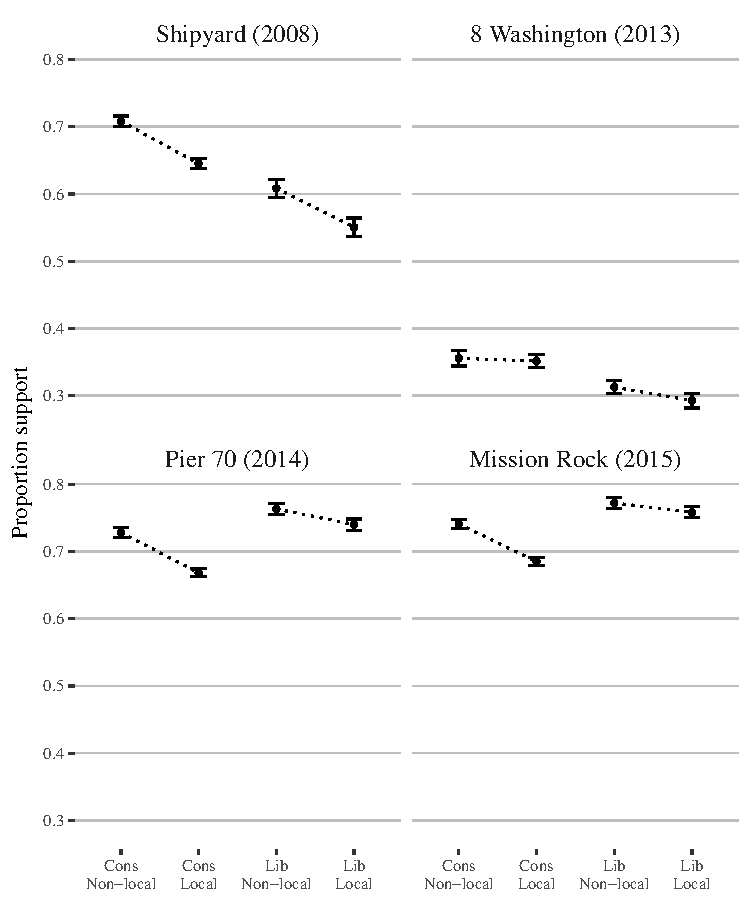
\includegraphics[width=.9\textwidth]{g_lib_loc}
  }
  \end{measuredfigure}
  \begin{tablenotes}[flushleft]
    \item \hspace{-.2em}\emph{Notes:} The figure shows the proportion of respondents that support each project type, for each liberalism-localism category. Error bars indicate 95\% confidence intervals.
  \end{tablenotes}
\end{figure}

\subsubsection{Alternative Measures of Liberalism and Localism}

Interpretations of the principal components are subjective. That is, although I show that the first and third PCs from a principal components analysis of ballot measure outcomes are systematically associated with vote outcomes for redevelopment projects in a manner consistent with expectations from a theory of liberalism and localism, interpretations of the PCs may differ across researchers.  

To address this concern, I use vote outcomes on individual ballot propositions as measures of liberalism and localism.  I select propositions that express liberalism and localism with the least ambiguity.  To measure liberalism, I use precinct-level vote shares for November 2015 Proposition A. The proposition sought voter approval to borrow \$310 million for the development and preservation of low- and middle-income housing, as well as financial assistance for middle-income homebuyers. To measure localism, I use vote shares for Proposition J, ``Legacy Business Historic Preservation Fund,'' from the same election.  The fund would provide subsidies to legacy businesses, defined as businesses that have been operating in San Francisco for at least 20 years and ``have significantly contributed to history or identity of a neighborhood.''  The proposition does not raise new taxes or identify funding sources, but clearly expresses a preference for local and long-time businesses over newcomers.

Figure~\ref{fig:g_contour} shows how support for the Pier 70 and Mission Rock projects varies with vote shares for Propositions A and J.  As in Figure~\ref{fig:e_contour}, I use local regression to fit support for each redevelopment project to vote shares for Propositions A and J, and plot predicted vote shares over a range of values for both regressors.  Recall that both Pier 70 and Mission Rock projects had relatively high proportions of housing units set aside for low- and middle-income households.  Predicted vote shares for both projects increase from the top left corner (low liberalism, high localism) to the bottom right corner (high liberalism, low localism).  These results echo those from the bottom panel of Figure~\ref{fig:g_lib_loc}.  In particular, the localism gradients of support for both projects are relatively shallow among liberals. That is, among liberal precincts, low-localism and high-localism neighborhoods are similarly supportive of both the Pier 70 and Mission Rock projects.  Indeed, predicted support for the Mission Rock project is highest in the top right corner, i.e. among liberal precincts with high localism scores.  The findings suggest that support for redevelopment projects, even among localist neighborhoods, can be conditional on features of the development.  Opposition to development need not be a matter of unyielding dogma.

\begin{figure}[t]
  \caption{Contour Plots of Support for Projects}
  \label{fig:g_contour}
  \begin{measuredfigure}
  \makebox[\linewidth]{%
  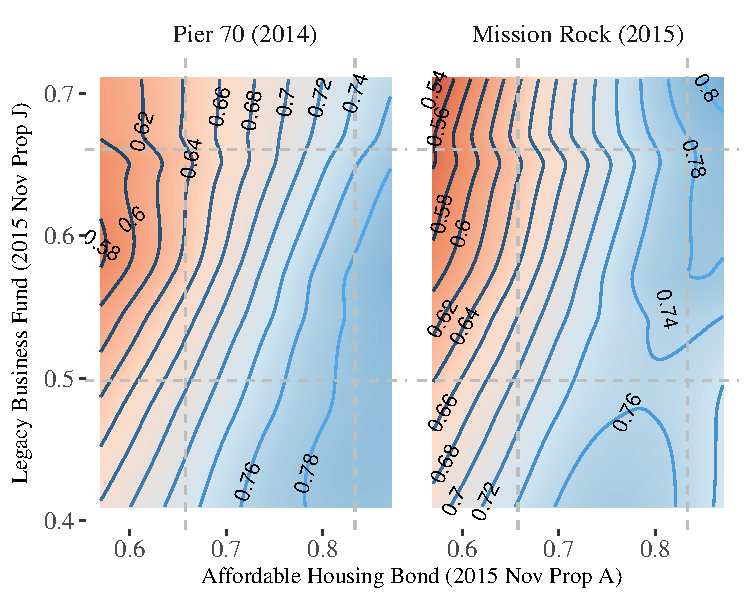
\includegraphics[width=.85\textwidth]{g_contour}
  } 
  \end{measuredfigure}
  \begin{tablenotes}[flushleft]
    \item \hspace{-.2em}\emph{Notes:} The figure reports predicted support for the Pier 70 and Mission Rock projects from loess estimates.  Levels of predicted support are indicated by colors in the plot as well as labels on the contour lines.  The predictors are the proportion of votes in each precinct supporting 2015 November Prop A (Affordable Housing Bond) and Prop J (Legacy Business Fund).  The vertical and horizontal dashed lines represent the 20th and 80th percentiles for the proportion of votes supporting the propositions.
  \end{tablenotes}
\end{figure}

\section{Discussion}\label{sec:discussion}

The model in this paper presents a way to understand support for housing growth in dense, urban areas.  Liberals who oppose new residential development do not do so because they are misinformed or hypocritical. Instead, liberalism should be understood as a preference for redistribution and economic equity.  Liberalism in this sense does not imply support for social inclusion broadly considered; it is limited to an aversion to economic inequity. Support for redevelopment projects increases with liberalism when benefits of the project are perceived to be distributed equitably. In short, liberals do not see housing growth as a phenomenon to be supported or opposed always and everywhere.

The model also gives localism a role in shaping support for development.  The costs of development, such as traffic congestion and the loss of natural or cultural amenities, are borne by local neighbors, and may not necessarily be mitigated by the benefits of development.  Localism that gives rise to anti-development sentiments cannot be mitigated by redistributing the benefits of development among income groups.  Localism's association with opposition to residential development may be attenuated if planners and developers enter into good-faith consultations with local community groups. Systematic analysis of this hypothesis is left for future work, but \citet{kuwada_shaping_2015} persuasively argues that community engagement was critical for gaining the necessary approvals in the case of Pier 70.

These results offer implications about the efficacy of measures to engender support for new residential development.  \citet{fischel_why_2001} begins from the premise that homeowners fear changes to the neighborhood could erode the value of their homes, and proposes a variety of financial innovations that could mitigate these concerns.  The findings from this paper suggest why measures to protect housing wealth may be ineffective in boosting support for new development. If objections to new market-rate development among city dwellers are motivated by sincere concerns about economic equity, then they are unlikely to be overcome by home price guarantees.  

In this respect, inclusionary zoning laws -- requirements that a proportion of new housing units be set aside for low- or middle-income households -- may help to ease the politics of development, in cities where local residents are already favorably predisposed to redistributive public policy.  Whether inclusionary zoning laws promote housing affordability is a matter of some debate. There is agreement that inclusionary zoning rules result in the production of more housing units deemed affordable. But some point out that because affordable set-asides are a tax on market-rate units, inclusionary zoning rules may reduce the overall level of housing production \citep[p. 82]{glaeser_rethinking_2008}. At the same time, local political opposition to new development also imposes tangible costs on developers, for example when local institutions allow opponents to frustrate and delay development.  To the extent that the economic tax imposed by inclusionary zoning laws is offset by easier passage of a project through the political process, inclusionary zoning may promote housing production overall.  Planners and developers are likely to find most success when projects are consistent with the political dispositions of local constituencies.

Finally, this study foregrounds the role of localism in shaping attitudes toward residential development. Localism should not be conflated with dogmatic opposition to local development. Analysis of redevelopment projects in San Francisco shows variation in the association between localism and support for these projects. More precise conceptualization and measurement of localism would advance the understanding of support for housing growth of different kinds. For instance, a localism that privileges current residents may have different implications for attitudes toward housing growth than a localism that favors community members broadly considered, including non-residents who serve local communities.  As a political issue, urban redevelopment relates to strongly held conceptions of community identity and neighborhood character, as well as beliefs about access to and exclusion from the urban commons.  Research on attitudes toward housing growth will play a valuable role in informing the practice of urban development, at a time when so many are seeking to participate in urban life.


% =============================================================================
% References
% =============================================================================

\bibliography{/Users/weihuang/Documents/latex/my_library}

% =============================================================================
% Appendices
% =============================================================================

\clearpage

\appendix
\renewcommand\thefigure{\thechapter.\arabic{figure}}    
\renewcommand\thetable{\thechapter.\arabic{table}}

\chapter*{Appendix}
\setcounter{chapter}{1}
\setcounter{figure}{0}
\setcounter{table}{0}

\section{Political Beliefs}\label{sec:e_political_beliefs}

The following attitudinal questions were used to construct composite measures of liberalism and localism.  Each set of statements appears on a different page in the survey.

\vspace{1em}\noindent \emph{Set 1:}
\begin{enumerate}
  \item The distribution of money and wealth in this country today is fair.
  \item It is the government's duty to make sure everyone can afford decent housing.
  \item Local government should focus on helping local businesses do well, rather than attracting new firms to the area.
  \item The government should not concern itself with reducing the income difference between the rich and the poor.
\end{enumerate}

\noindent \emph{Set 2:}
\begin{enumerate}
  \setcounter{enumi}{4}
  \item Big business has too much influence over the decisions made by our government today.
  \item Our government should redistribute wealth through higher taxes on the rich.
  \item It is not the local government's job to regulate home prices and rents in my town or city.
  \item Corporations should focus on making money for their shareholders, rather than being socially responsible.
\end{enumerate}

\noindent \emph{Set 3:}
\begin{enumerate}
  \setcounter{enumi}{8}  
  \item Everyone born in this country has an equal chance to succeed in life, whether their family is rich or poor.
  \item On balance, the free market is the fairest way to allocate housing.
  \item People who cannot afford their rent should move to somewhere cheaper, instead of asking the government for help.
  \item Every resident of a town or city should have an equal say on local issues, whether they just arrived or are long-time residents.
\end{enumerate}

\clearpage
\section{Figures and Tables}

\begin{figure}[htb]\centering
  \caption{Average Treatment Effects by Liberalism and Localism Scores}
  \label{fig:e_ate}
  \begin{measuredfigure}
  \makebox[\linewidth]{%
  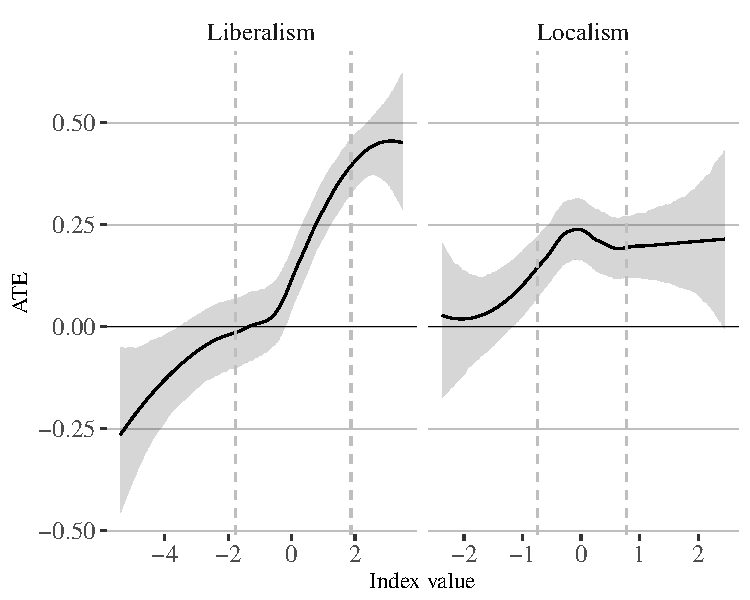
\includegraphics[width=.85\textwidth]{e_ate}
  }  
  \end{measuredfigure}
  \begin{tablenotes}[flushleft]
    \item \hspace{-.2em}\emph{Notes:} The figure shows the average treatment effect (ATE), or the relative preference for the mixed-income project over the high-end project, across a range of liberalism and localism scores.  The ATE corresponds to the difference between the loess curves reported in Figure~\ref{fig:e_lib_loc}.  The support (range) for each plot consists of values between the 1st and 99th percentiles for each index.  Shaded areas indicate 95\% confidence intervals. The vertical dashed lines represent the 20th and 80th percentiles for the respective scores.
  \end{tablenotes}
\end{figure}

\begin{table}
  \caption{Regressions of Support for Project on Liberalism and Localism}
  \label{tab:e_support_regression}
  \begin{threeparttable}
  \scriptsize
  \begin{tabularx}{\linewidth}{X}
  \centering

  \begin{tabular}{@{\extracolsep{5pt}}lcccc} 
  \\[-1.8ex]\hline 
  \hline \\[-1.8ex] 
   & \multicolumn{4}{c}{\textit{Dependent variable:}} \\ 
  \cline{2-5} 
  \\[-1.8ex] & High-end & Mixed-income & High-end & Mixed-income\\ 
  \\[-1.8ex] & (1) & (2) & (3) & (4)\\ 
  \hline \\[-1.8ex] 
   Liberalism & $-$0.045$^{}$ & 0.050$^{}$ & $-$0.040$^{}$ & 0.049$^{}$ \\ 
    & (0.008) & (0.007) & (0.008) & (0.008) \\ 
    & & & & \\ 
   Liberalism-squared & $-$0.006$^{}$ & $-$0.002 & $-$0.006$^{}$ & $-$0.003 \\ 
    & (0.003) & (0.003) & (0.003) & (0.003) \\ 
    & & & & \\ 
   Localism & $-$0.088$^{}$ & $-$0.041$^{}$ & $-$0.077$^{}$ & $-$0.043$^{}$ \\ 
    & (0.015) & (0.014) & (0.016) & (0.015) \\ 
    & & & & \\ 
   Localism-squared & 0.005 & 0.001 & 0.004 & 0.005 \\ 
    & (0.010) & (0.010) & (0.010) & (0.010) \\ 
    & & & & \\ 
   Female &  &  & $-$0.104$^{}$ & 0.002 \\ 
    &  &  & (0.032) & (0.029) \\ 
    & & & & \\ 
   White &  &  & 0.010 & 0.058$^{}$ \\ 
    &  &  & (0.037) & (0.034) \\ 
    & & & & \\ 
   Age < 35 &  &  & $-$0.022 & 0.010 \\ 
    &  &  & (0.034) & (0.031) \\ 
    & & & & \\ 
   No 4-year college degree &  &  & $-$0.025 & $-$0.008 \\ 
    &  &  & (0.035) & (0.031) \\ 
    & & & & \\ 
   Post-graduate degree &  &  & $-$0.005 & $-$0.035 \\ 
    &  &  & (0.047) & (0.046) \\ 
    & & & & \\ 
   Income < \$60,000 &  &  & $-$0.082$^{}$ & 0.043 \\ 
    &  &  & (0.038) & (0.034) \\ 
    & & & & \\ 
   Income \$100-150,000 &  &  & 0.009 & 0.018 \\ 
    &  &  & (0.055) & (0.049) \\ 
    & & & & \\ 
   Income > \$150,000 &  &  & 0.086 & 0.093 \\ 
    &  &  & (0.078) & (0.082) \\ 
    & & & & \\ 
   Homeowner &  &  & $-$0.013 & $-$0.031 \\ 
    &  &  & (0.036) & (0.032) \\ 
    & & & & \\ 
   Resident > 4 years &  &  & $-$0.032 & $-$0.006 \\ 
    &  &  & (0.035) & (0.031) \\ 
    & & & & \\ 
   5-year HPA > median &  &  & $-$0.033 & 0.007 \\ 
    &  &  & (0.032) & (0.029) \\ 
    & & & & \\ 
   Constant & 0.561$^{}$ & 0.730$^{}$ & 0.720$^{}$ & 0.668$^{}$ \\ 
    & (0.022) & (0.020) & (0.066) & (0.060) \\ 
    & & & & \\ 
  \hline \\[-1.8ex] 
  Observations & 1,007 & 982 & 970 & 971 \\ 
  R$^{2}$ & 0.062 & 0.072 & 0.085 & 0.080 \\ 
  Adjusted R$^{2}$ & 0.058 & 0.068 & 0.071 & 0.066 \\ 
  \hline 
  \hline \\[-1.8ex] 
  \end{tabular}   

  \end{tabularx}
  \begin{tablenotes}[flushleft]
    \item \hspace{-.2em}\emph{Notes:} OLS estimates of linear probability models for project support.
  \end{tablenotes}
  \end{threeparttable}
\end{table}

\begin{figure}[htb]\centering
  \caption{Proportion of Variance Explained}
  \label{fig:g_scree}
  \begin{measuredfigure}
  \makebox[\linewidth]{%
  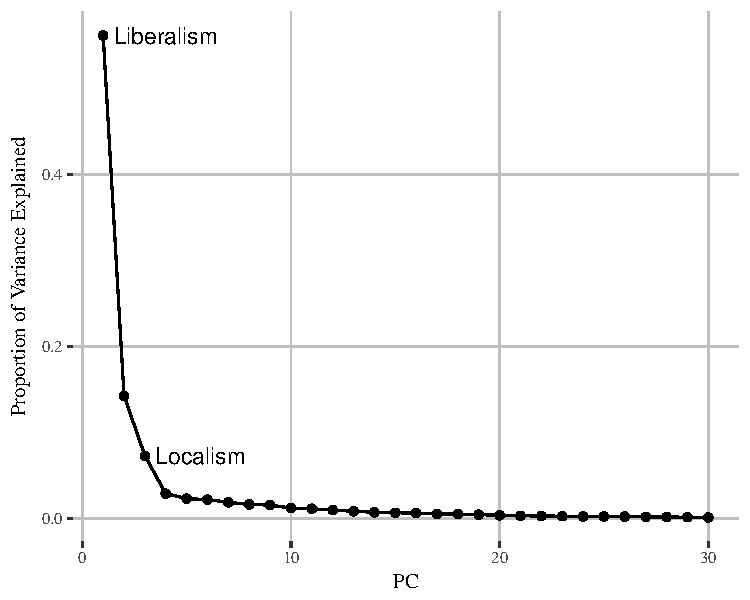
\includegraphics[width=.85\textwidth]{g_scree}
  }  
  \end{measuredfigure}
  \begin{tablenotes}[flushleft]
    \item \hspace{-.2em}\emph{Notes:} The figure shows the proportion of variance explained by each principal component.
  \end{tablenotes}
\end{figure}

\begin{table}
  \caption{Regressions of Support for Project on Liberalism and Localism}
  \label{tab:g_support_regression}
  \begin{threeparttable}
  \scriptsize
  \begin{tabularx}{\linewidth}{X}
  \centering

  \begin{tabular}{@{\extracolsep{5pt}}lcccc} 
  \\[-1.8ex]\hline 
  \hline \\[-1.8ex] 
   & \multicolumn{4}{c}{\textit{Dependent variable:}} \\ 
  \cline{2-5} 
  \\[-1.8ex] & Shipyard & 8 Wash. & Pier 70 & Mission Rock\\ 
  \\[-1.8ex] & (1) & (2) & (3) & (4)\\ 
  \hline \\[-1.8ex] 
   Localism & $-$0.037$^{}$ & $-$0.012$^{}$ & $-$0.021$^{}$ & $-$0.021$^{}$ \\ 
    & (0.003) & (0.003) & (0.002) & (0.002) \\ 
    & & & & \\ 
   Liberalism & $-$0.063$^{}$ & $-$0.028$^{}$ & 0.033$^{}$ & 0.022$^{}$ \\ 
    & (0.003) & (0.003) & (0.002) & (0.002) \\ 
    & & & & \\ 
   Constant & 0.642$^{}$ & 0.353$^{}$ & 0.714$^{}$ & 0.765$^{}$ \\ 
    & (0.006) & (0.007) & (0.004) & (0.004) \\ 
    & & & & \\ 
  \hline \\[-1.8ex] 
  Strata fixed effects & Yes & Yes & Yes & Yes \\ 
  \hline \\[-1.8ex] 
  Observations & 569 & 569 & 569 & 569 \\ 
  R$^{2}$ & 0.641 & 0.219 & 0.586 & 0.614 \\ 
  Adjusted R$^{2}$ & 0.635 & 0.205 & 0.579 & 0.607 \\ 
  \hline 
  \hline \\[-1.8ex] 
  \end{tabular} 

  \end{tabularx}
  \begin{tablenotes}[flushleft]
    \item \hspace{-.2em}\emph{Notes:} OLS estimates of linear models for project support. Coefficients for localism and liberalism represent change in vote share for a standard deviation change in the predictor value. Strata are generated by first computing terciles for precinct-level median household income and precinct-level homeownership rates, then interacting both categorical variables to form nine cells. Household income and homeownership rates come from the 2010 Census, and are imputed to precincts from Census geographies using conversion tables from the Statewide Database, available at \url{http://statewidedatabase.org/conversion.html}.
  \end{tablenotes}
  \end{threeparttable}
\end{table}

\end{document}